\section{Magnetic Resonance Imaging}
 \subsection{Magnetic properties of nuclei}
 Biological organisms and tissues are naturally abundant of \emph{Hydrogen} atoms, mostly in water and fats. Thanks to the magnetic properties of Hydrogen atoms it is possible to build anatomical images of the human body.

 From a classical point of view an atomic nucleus can be assumed as sphere rotating around its axis \ref{fig:spin_proton}. This rotation is called spin and it is a fundamental property of nucleus. The \emph{spin} is the intrinsic angular momentum of the nucleus and can be an integer or a half-integer depending of the mass number\footnote{Mass number: number of protons and neutrons} and the atomic number\footnote{Atomic number: number of protons}. In the particular case of the Hydrogen it is present only a proton and the spin can take only tha values $1/2$ and $-1/2$. \cite{slides} \\
 Since the nucleus is a charged particle, a rotation of it creates a magnetic field. From this point of view the particle behaves like a small magnetic dipole \ref{fig:spin_proton}: $ \vec{\mu} =i\mathbf{S}$ where $\vec{\mu}$ is the intrinsic magnetic momentum that is aligned on its spin $\mathbf{S}$.

 \begin{figure}
   \centering
   \begin{subfigure}{.4\textwidth}
     \centering
     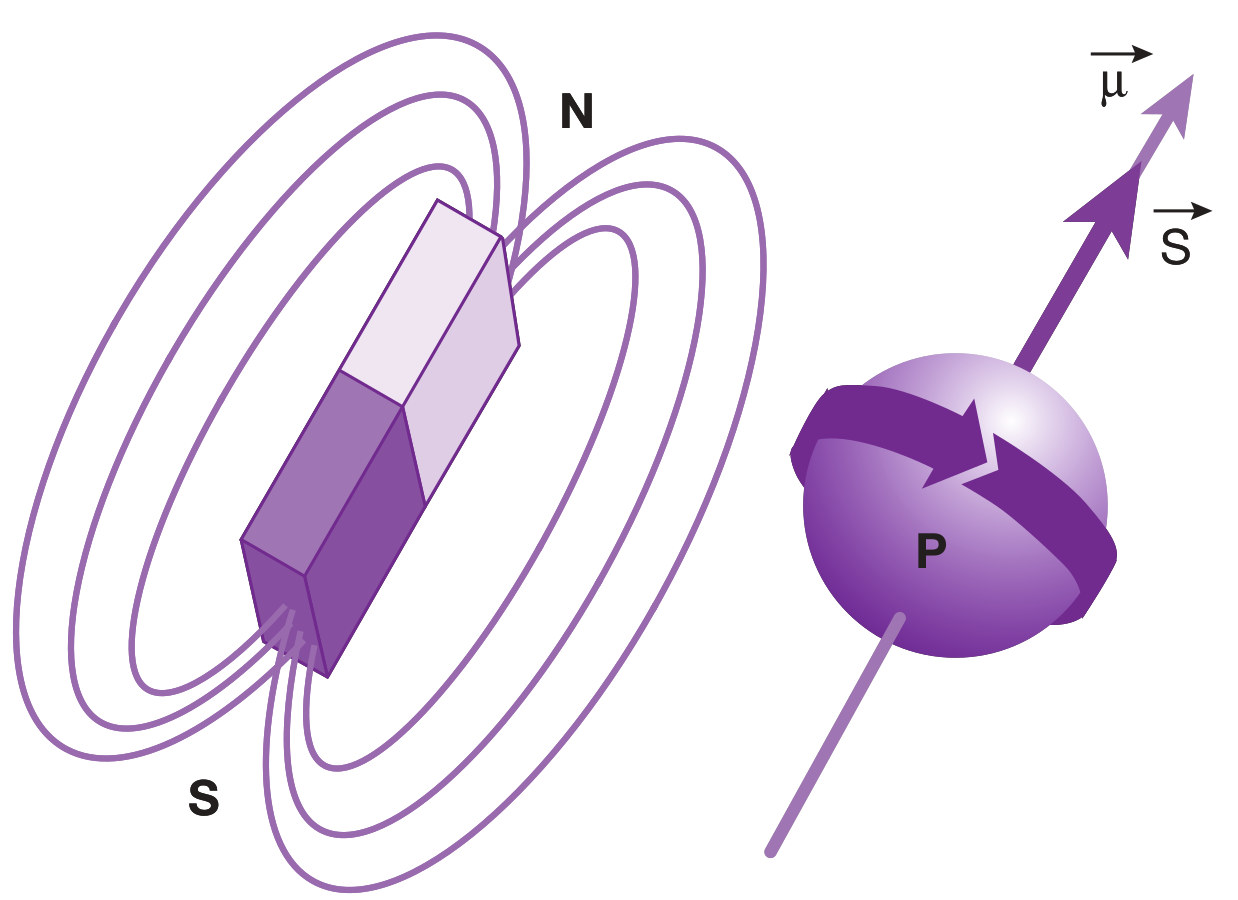
\includegraphics[width=0.7\linewidth]{images/magnetic_dipole.png}
     \caption{}
     \label{fig:spin_proton}
   \end{subfigure}%
   \begin{subfigure}{.6\textwidth}
     \centering
     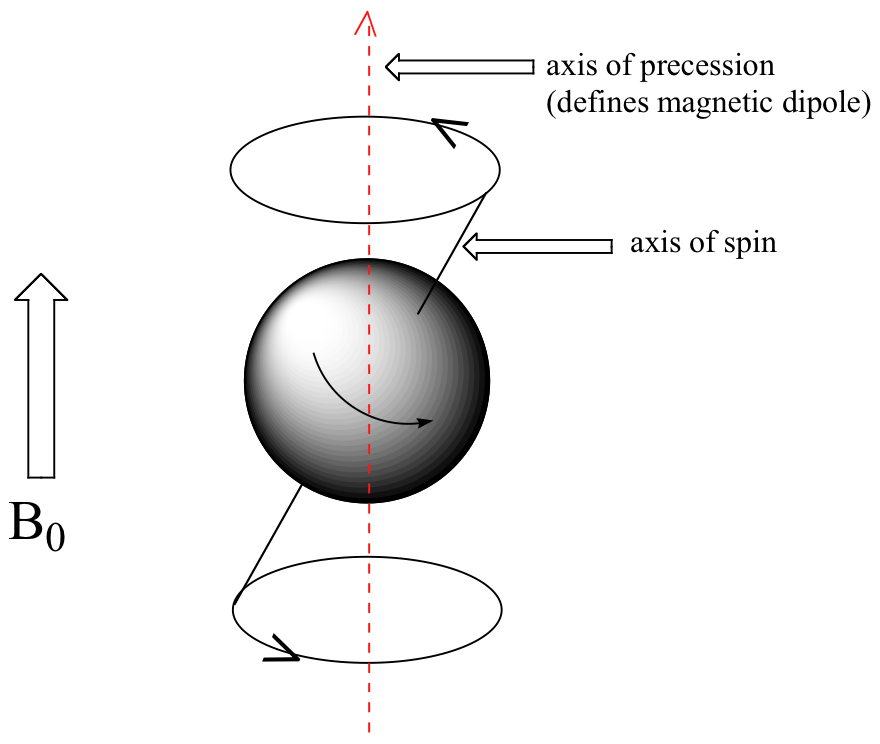
\includegraphics[width=0.7\linewidth]{images/precession.png}
     \caption{}
     \label{fig:spin_precession}
   \end{subfigure}
   \caption{(a) Representation of the spin and the magnetic moment. \cite{KastlerVetterIRM}, (b) Precessional motion of a proton spin in an applied magnetic field. \cite{organicChemestry}}
\end{figure}

 \noindent Normally orientation of $\vec{\mu}$ is completely random due to thermal random motion, therefore the sum of the magnetic fields is null ($\sum_{i} \mu_{i} = 0$). \\
 In a magnetic dipole, when an external magnetic field $\mathbf{B_{0}}$ is applied, the individual orientation can take two possible orientations: \emph{parallel} or \emph{anti-parallel}. This phenomena in the particles is different, since the particle is rotating, the external magnetic field creates a \emph{precession} around $\mathbf{B_{0}}$ like a spinning top \ref{fig:spin_precession}: $\mathbf{\Gamma}=\vec{\mu} \times \mathbf{B_{0}}$ where $\mathbf{\Gamma}$ is the \emph{torque}. The axis rotates around the area of a "cone", with an angular speed proportional to the applied field following the \emph{Larmor's Law}:
 \begin{equation}
    f_{0}=\frac{\gamma}{2\pi} B_{0}
 \end{equation}
 $\gamma$ is the gyromagnetic ratio and it is a characteristic of the nucleus. The frequency of precession is called \emph{Larmor frequency}.\\
 From a global point of view, the populations of protons moments create a macroscopic magnetization, with the direction equal to the external field \ref{fig:macroscopic_magnetization}, defined by \cite{slides}.
 \begin{equation}
    \mathbf{M}=\frac{1}{V}\sum_{i} \vec{\mu_{i}}
 \end{equation}
 While the transversal magnetization in $xy$ plane is null, since the components $\mu_{xy}$ rotate with different phases and overall they nullifying themselves \ref{fig:macroscopic_magnetization}.

 \begin{figure}[h]
    \centering
    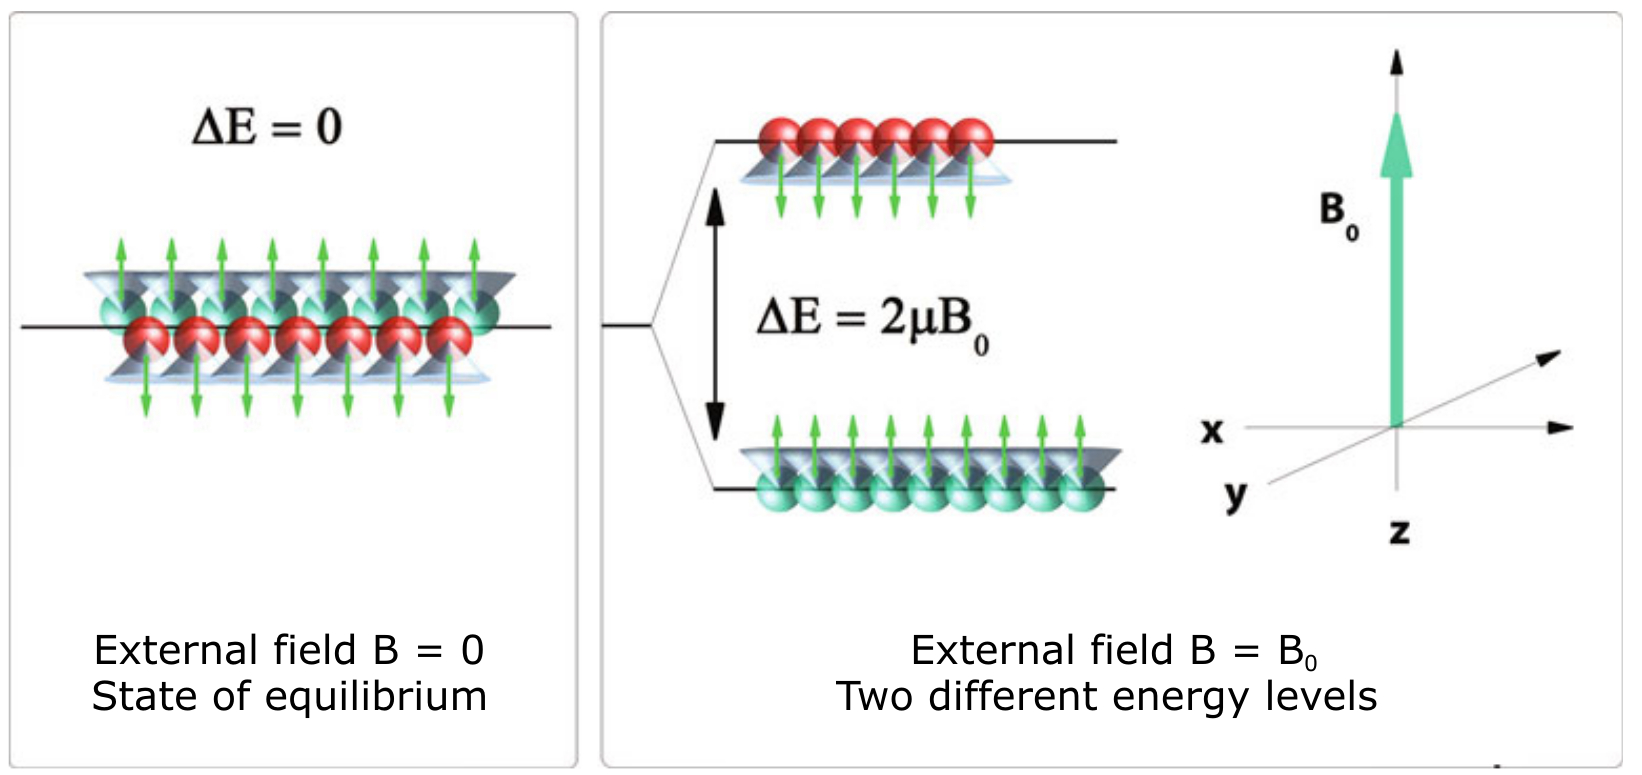
\includegraphics[width=0.8\textwidth]{images/energy_protons.jpg}
    \caption{Separation of different energy levels after the application of the external field $B_0$. The population of spins in the lower level is slightly more of the upper.\cite{elementiRisonanza} Translated.}
    \label{fig:macroscopic_magnetization}
 \end{figure}

 \noindent In terms of energy, without the magnetic field, it doesn't exists any difference between the two orientations (parallel and anti-parallel), because them are equiprobable. With the application of the static magnetic field the anti-parallel orientation will have an higher energy ($N\downarrow$) than the parallel with lower energy ($N\uparrow$), since it has to be the opposite of the external field. The \emph{occupation ratio} of the two energy levels is described by the \emph{Boltzmann distribution}.
 \begin{equation}
    \frac{N_\uparrow}{N_\downarrow}=e^{-\frac{\Delta E}{k T}}
 \end{equation}
 where $k$ is the Boltzmann's constant and $T$ is the absolute temperature in [K].\\
 The energy of a magnetic dipole in a magnetic field $\mathbf{B_0}$ can be defined by:
 \[E=-\vec{\mu}\cdot\mathbf{B_0}=-\mu_z B_0 \Rightarrow\]
 where $\mu_z=\gamma\frac{h}{2\pi}I$ 
 \[\Rightarrow E_I=-\gamma\frac{h}{2\pi}I B_0\]
 where $h$ is the Planck's constant and $I$ is the spin orientation for the Hydrogen.
 Knowing that:
 \[\Delta E=E_{-\frac{1}{2}} - E_{\frac{1}{2}} = h\frac{\gamma}{2\pi}B_0 = h f_0\]
 we find that there are more spins in $E_\uparrow$ (lower energy) state than $E_\downarrow$ (higher energy) state \ref{fig:macroscopic_magnetization}.\\
 The equilibrium macroscopic magnetization is non-zero and is defined by \cite{slides}:
 \begin{equation}
    M_0=\frac{(\frac{\gamma}{2\pi})^{2}h^{2}\rho B_{0}I (I+1)}{3kT}
 \end{equation}
 where $\rho$ is the spin density\footnote{Spin density: number of spins per unit volume} and $I = 1/2$ for Hydrogen.

 \subsection{Radiofrequency pulse}
 Since the intensity of the macroscopic magnetization ($M_0$) is several orders of magnitude smaller than the main field ($B_0$), is impossible to measure it directly\footnote{Even if is impossible to measure directly the $M_0$, it is proportional to the field, therefore an higher $B_0$ allows to generate higher signals with higher SNR and less acquisition times.}.\\
 The idea is to induce controlled oscillations of the spin system in order to generate a measurable signal as defined by \cite{slides}. If a RF pulse is applied at the Larmor frequency ($f_{RF} = f_0$) we observe a \emph{condition of resonance} \ref{fig:trajectory_magnetization}, and if the system resonates with the pulse it starts to absorb energy \ref{fig:energy_gaining} .
 \begin{equation}
    B_{1}(t)=2B_{1}(t)\cos(2\pi f_{RF}t+\phi)\mathbf{1_{xy}}
 \end{equation}

 \begin{figure}[h]
   \centering
   \begin{minipage}[c]{0.5\textwidth}
      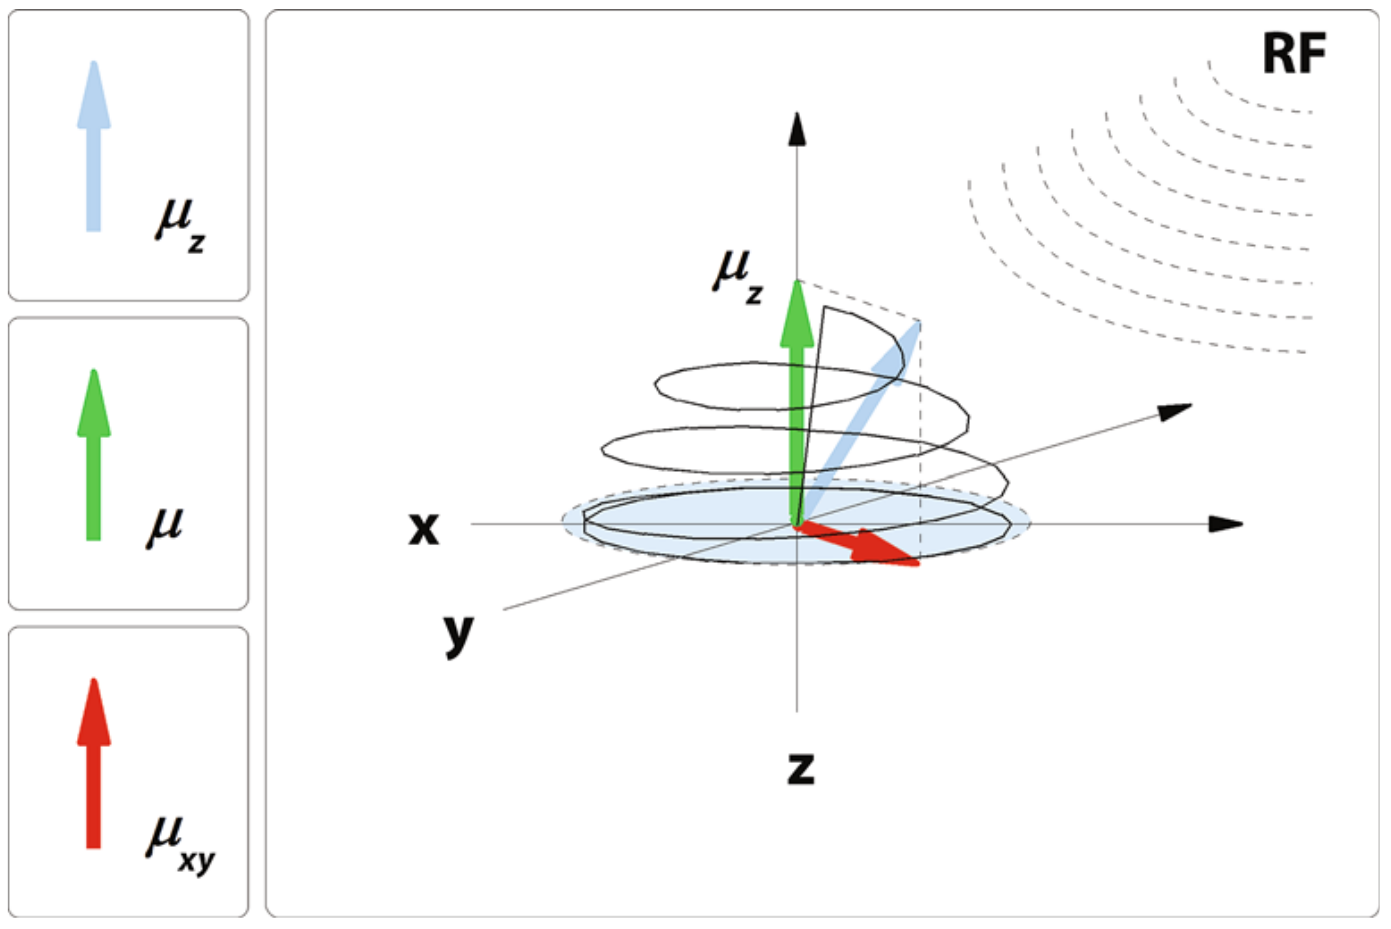
\includegraphics[width=\textwidth]{images/trajectory_magnetization.png}
   \end{minipage}\hfill
   \begin{minipage}[b]{0.45\textwidth}
      \caption{Trajectory of the magnetization vector. The vector describes a spiral trajectory by rotating at the Larmor frequency, tilting more and more, until it gets to rotate on the transverse plane. \cite{elementiRisonanza}}
      \label{fig:trajectory_magnetization}
   \end{minipage} 
 \end{figure}

 \begin{figure}[h]
    \centering
    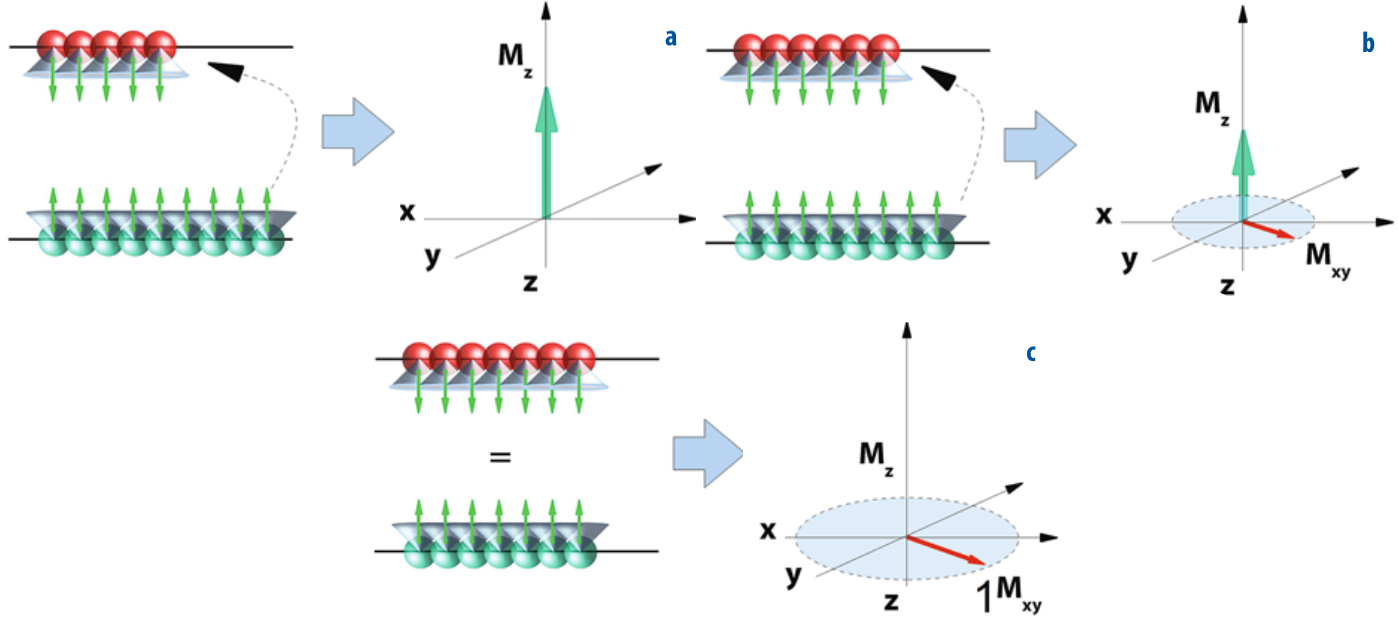
\includegraphics[width=0.9\textwidth]{images/energy_gaining.png}
    \caption{Effect of the RF impulse. (a) Initial situation; (b) System during the impulse; (c) System after 90 RF impulse. \cite{elementiRisonanza} Arranged.}
    \label{fig:energy_gaining}
 \end{figure}

 \noindent The \emph{flip angle} from the initial direction of the magnetization is defined by \cite{slides}:
 \[\theta = \gamma B_{1}T_{RF}\]
 where $T_{RF}$ is the duration of the RF-pulse.\\
 Now the magnetization vector can be represented with a longitudinal magnetization $M_z$ and a transverse magnetization $M_{xy}$ as in \cite{slides}:
 \begin{equation}
    \mathbf{M}=M_{z}\mathbf{1_{z}}+M_{xz}\mathbf{1_{xy}}
 \end{equation}

 \subsection{Relaxation}
 After applying the RF-pulse tends to go back to the initial state, these phenomena are called \emph{relaxation}. 
 \[M_{z} \rightarrow M_{0}\]
 \[M_{xy} \rightarrow 0 \]

 \begin{figure}[h]
   \centering
   \begin{minipage}[c]{0.5\textwidth}
      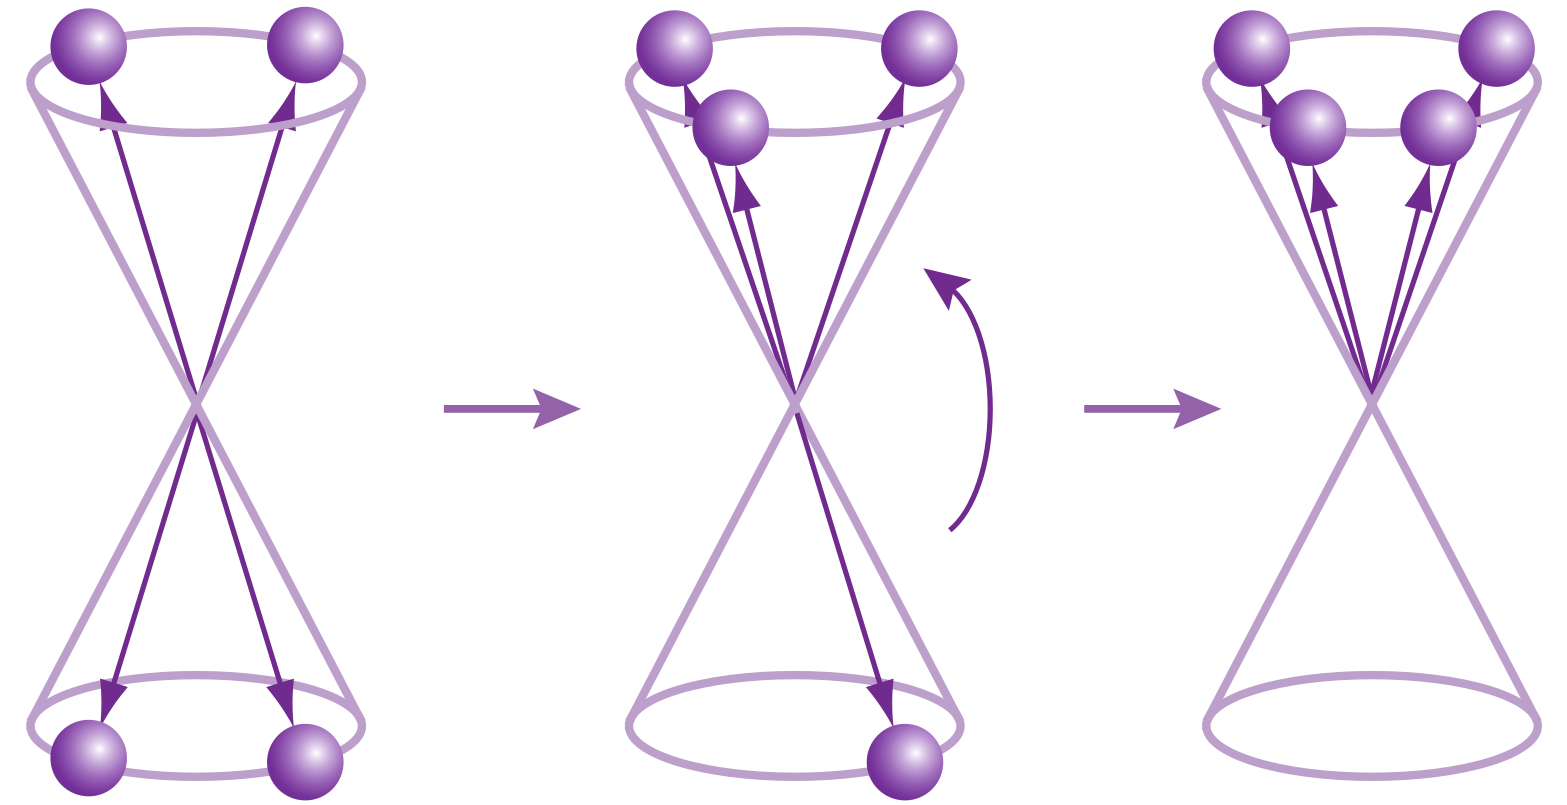
\includegraphics[width=\textwidth]{images/t1_relax_energy.png}
   \end{minipage}\hfill
   \begin{minipage}[b]{0.45\textwidth}
      \caption{There is a progressively transition to the equilibrium from the high level to the lower lever of energy. \cite{KastlerVetterIRM}}
      \label{fig:T1_relax_energy}
   \end{minipage}
 \end{figure}

 The first is the \emph{longitudinal relaxation} (\emph{spin-lattice relaxation} or \emph{T1-relaxation}) in which the magnetization recovers to its original $M_0$, because the energy state after the RF-pulse is unstable it will create a transition of spins from high energy to low energy \ref{fig:T1_relax_energy}. Can be mathematically descried by \cite{slides}:
 \begin{equation}
    M_{z}(t)=M_{0}+(M_{z}(0)-M_{0})e^{-\frac{t}{T_{1}}}
 \end{equation}
 where $T_1$ is the time needed to $M_{z}$ to reach the $63\%$ of the initial value $M_{0}$ \ref{fig:T1_relax_tissues}.
 
 \noindent In the T\textsubscript{1}-weighted image the signals must depend on the $T_1$ relaxation. Therefore the time between the RF-pulses have to be brief, but sufficient to differentiate the different tissues \ref{fig:T1_relax_tissues}. In these scans, the white matter is represented in light grey, the grey matter in a darker shade of grey and the fluids in black.

 % Qua l'immagine del libro ita 2.4
 \begin{figure}[h]
    \centering
    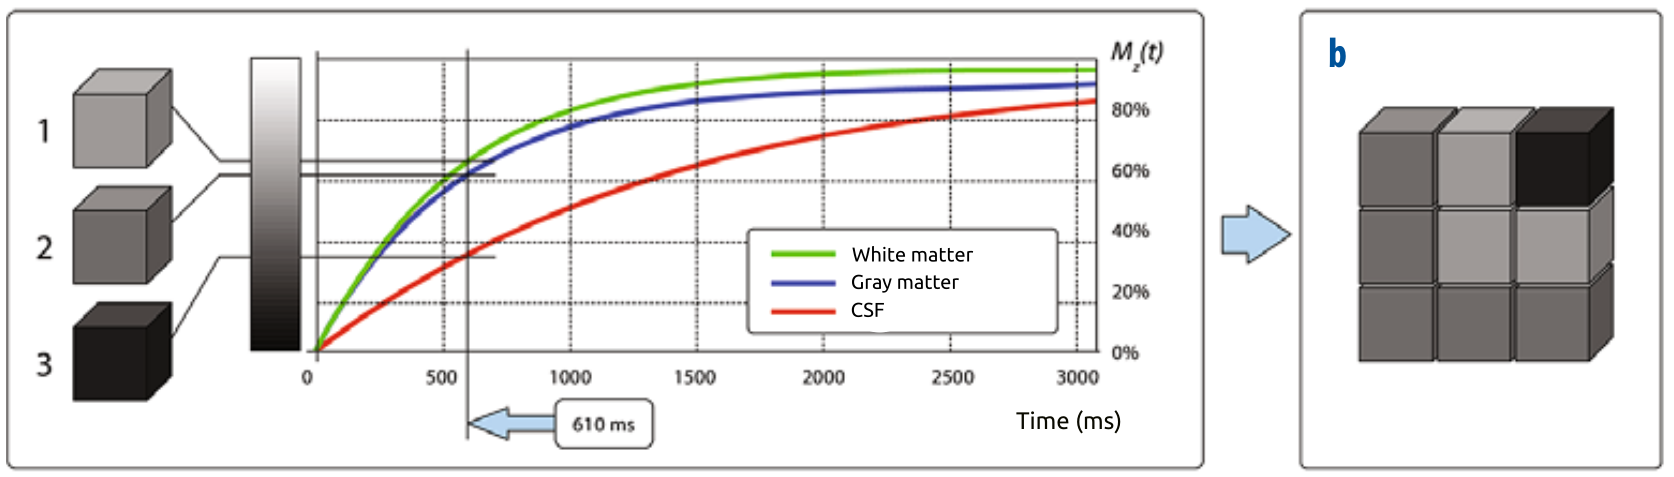
\includegraphics[width=1\textwidth]{images/t1_relax_tissues.png}
    \caption{The T\textsubscript{1} relaxation time is different for type of tissues. \cite{elementiRisonanza} Translated.}
    \label{fig:T1_relax_tissues}
 \end{figure}
 The second phenomenon is the \emph{transverse relaxation} (\emph{spin-spin relaxation} or \emph{T2-relaxation}) and it is characterized by a loss in coherence of the spin phases \ref{fig:T2_relax_phases}. It can be written as in \cite{slides}:
 \begin{equation}
    M_{xy}(t)=M_{xy}(0)e^{-\frac{t}{T_{2}}}
 \end{equation}
 where $T_2$ is the time needed to $M_{xy}$ to reduce itself to $37\%$ of the initial value \ref{fig:T2_relax_tissues}.

 \begin{figure}[h]
   \centering
   \begin{minipage}[c]{0.5\textwidth}
      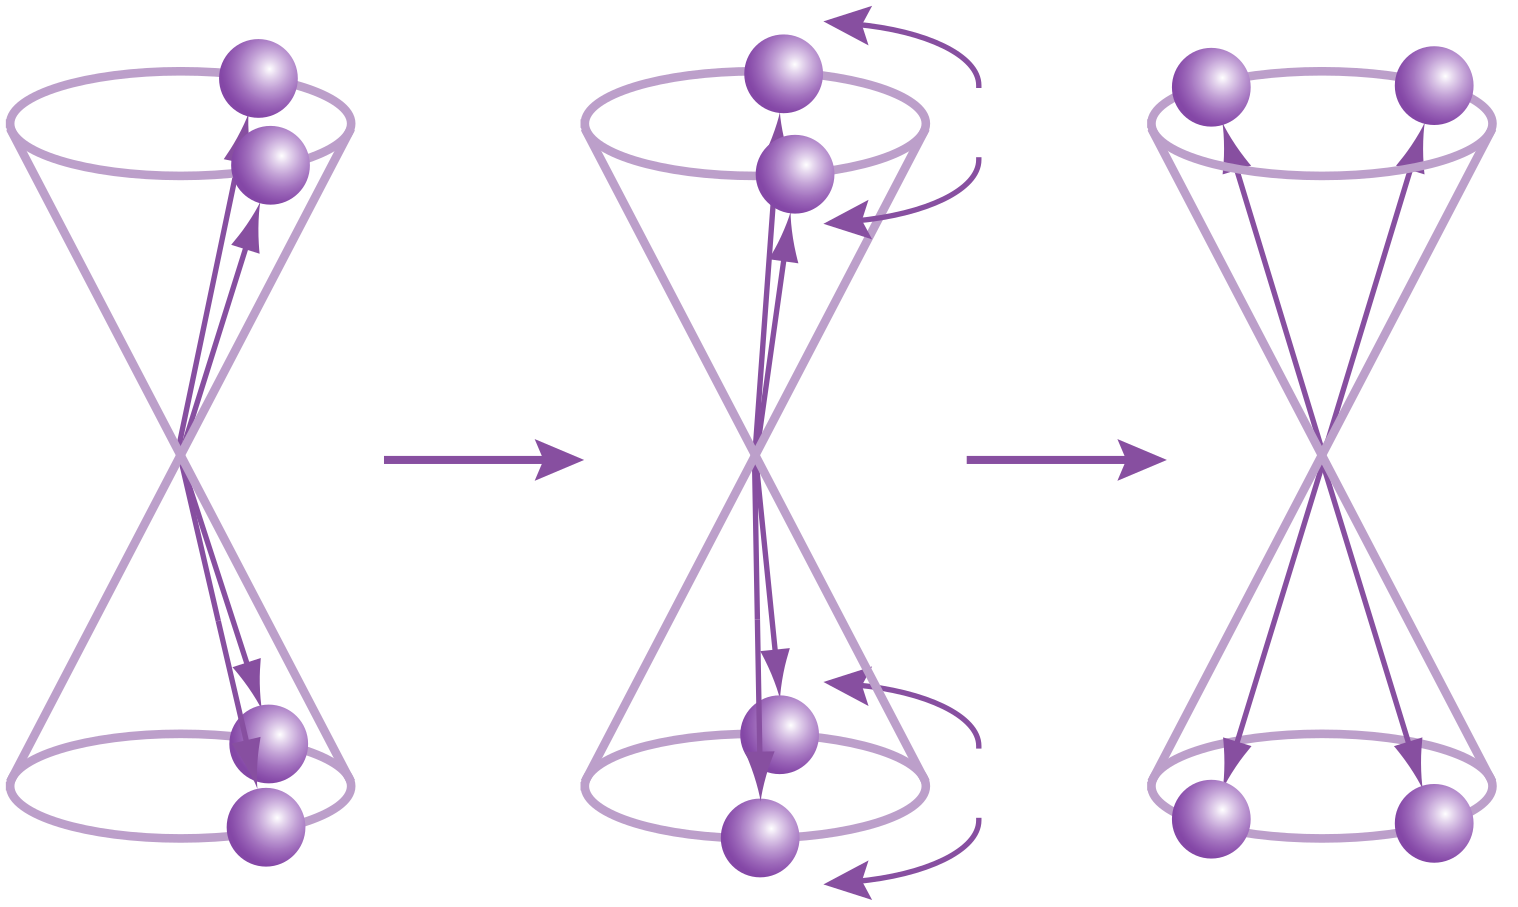
\includegraphics[width=1\textwidth]{images/t2_relax_phases.png}
   \end{minipage}\hfill
   \begin{minipage}[b]{0.45\textwidth}
      \caption{After the RF impulse there is a fast dephasing of the protons. The transversal magnetization $M_{xy}$ decreases quickly. \cite{KastlerVetterIRM} }
      \label{fig:T2_relax_phases}
   \end{minipage}
\end{figure}
 
 In the T\textsubscript{2}-weighted imaged the signals must depend only from the $T_2$ relaxation. Therefore is needed to wait that the $T_1$ relaxation effects are exhausted before reading the signal and send a new one. In these scans, the white matter is in dark grey, the grey matter is in light grey and the cerebrospinal fluid is in white \ref{fig:T2_relax_tissues}.

 % Qua l'immagine del libro ita 2.2
 \begin{figure}[h]
    \centering
    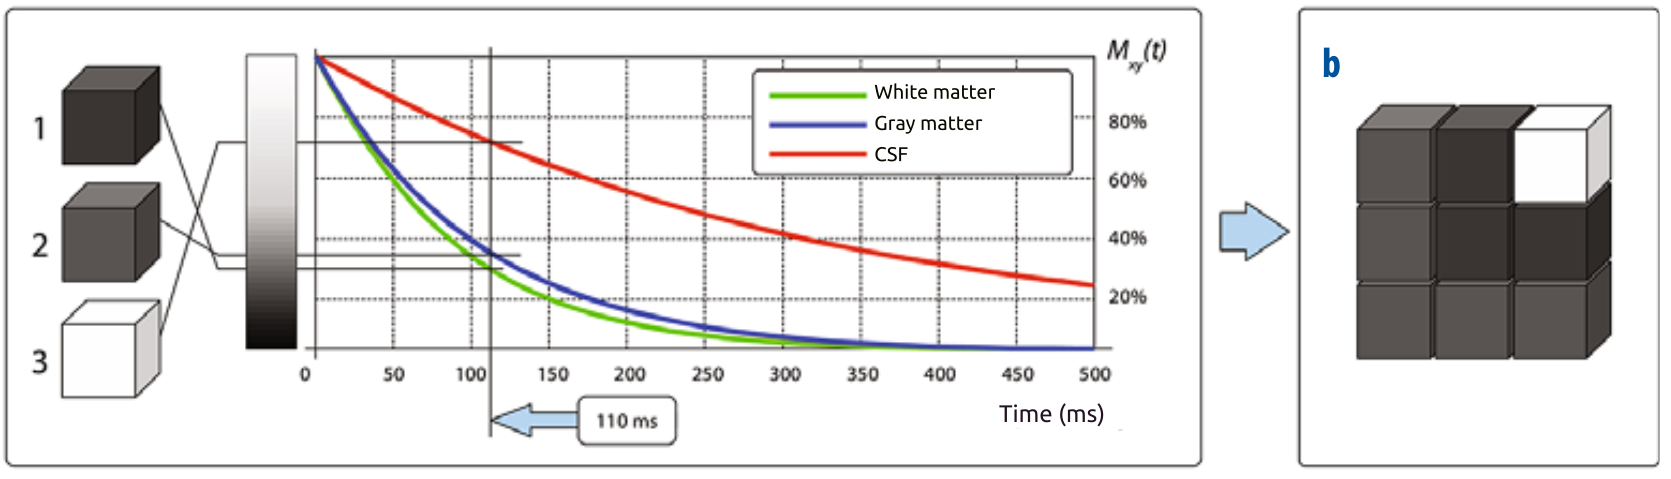
\includegraphics[width=1\textwidth]{images/t2_relax_tissues.png}
    \caption{The T\textsubscript{2} relaxation time is different for type of tissues. \cite{elementiRisonanza} Translated.}
    \label{fig:T2_relax_tissues}
 \end{figure}

 \noindent In real conditions of an imperfect homogeneity of the field $B_0$ we see the \emph{effective relaxation time}, define by \cite{slides}:
 \begin{equation}
    \frac{1}{T_{2}*} = \frac{1}{T_2}+\gamma\Delta B_0
 \end{equation}
 Where $\Delta B_0$ are the inhomogeneities in the magnetic field.

 \subsection{Spin-echo sequence}
 To obtain images with different type of contrast is needed to control the time between RF-pulses and the time of between readings of the signal. \\
 The first sequence utilized for clinical purpose is the \emph{spin-echo}. It introduces two main parameters: \emph{Echo time} ($TE$) and the \emph{Repetition time} ($TR$). The time between two 90° RF-pulses is defined ad $TR$, while the time between the RF-pulse and the first echo is defined as $TE$.\\
 The strength of this sequence is the capacity of reading the T\textsubscript{2}-weighted signals and not the T\textsubscript{2}* \ref{fig:T2vsT2*}.

 \begin{figure}[h]
    \centering
    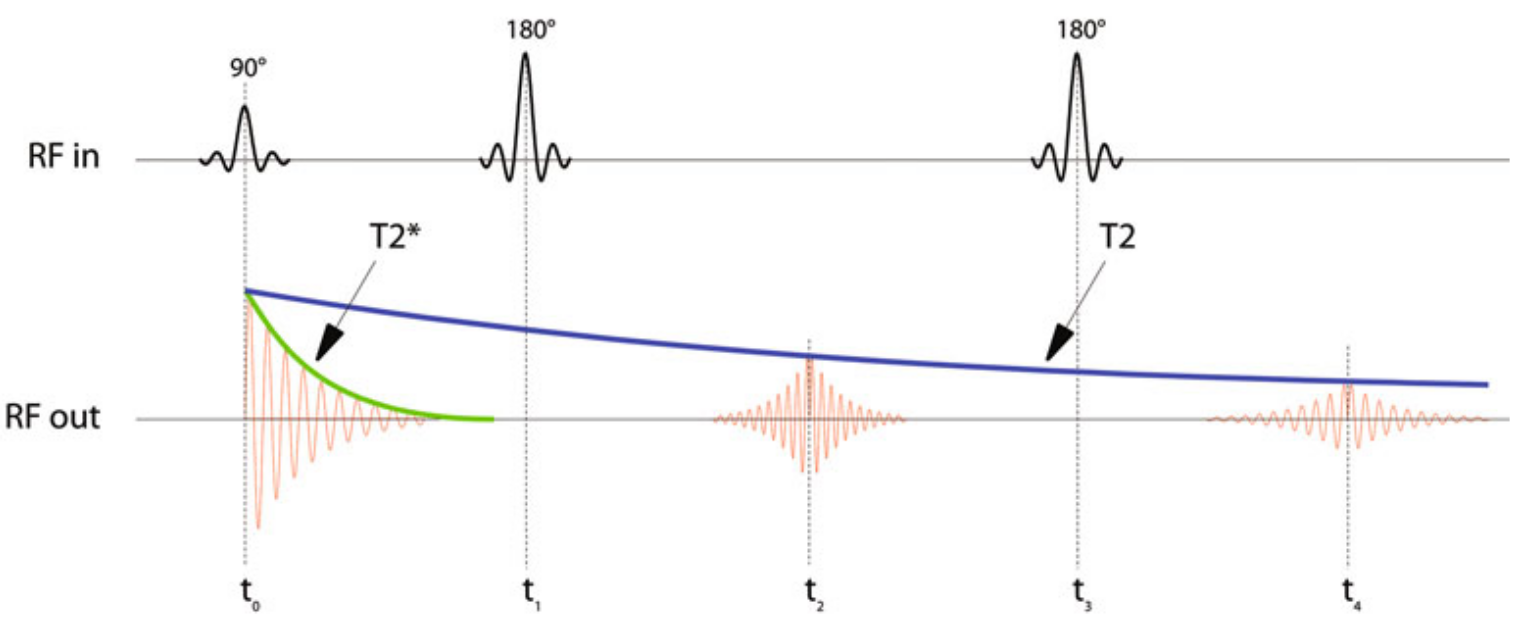
\includegraphics[width=1\textwidth]{images/t2vst2star.png}
    \caption{Recovering of the T\textsubscript{2}-weighted signals from the T\textsubscript{2}* through the Spin-echo sequence. The T\textsubscript{2}-weighted signals is created by interpolating the peaks of the spin echo signals. The time between $t_0$ and $t_2$ is defined ad $TE$ \cite{elementiRisonanza}}
    \label{fig:T2vsT2*}
 \end{figure}

 \noindent The spin-echo sequence is composed of two type of RF-pulses: a 90° pulse and many 180° pulses. These last pulses have a double intensity and are called \emph{echo impulses}. An echo impulse mirror all the spins of 180°, therefore the faster spins and the slower are inverted of position, creating the possibility that all the spins are refocused at time $TE$. \cite{slides}

 \begin{figure}[h]
   \centering
   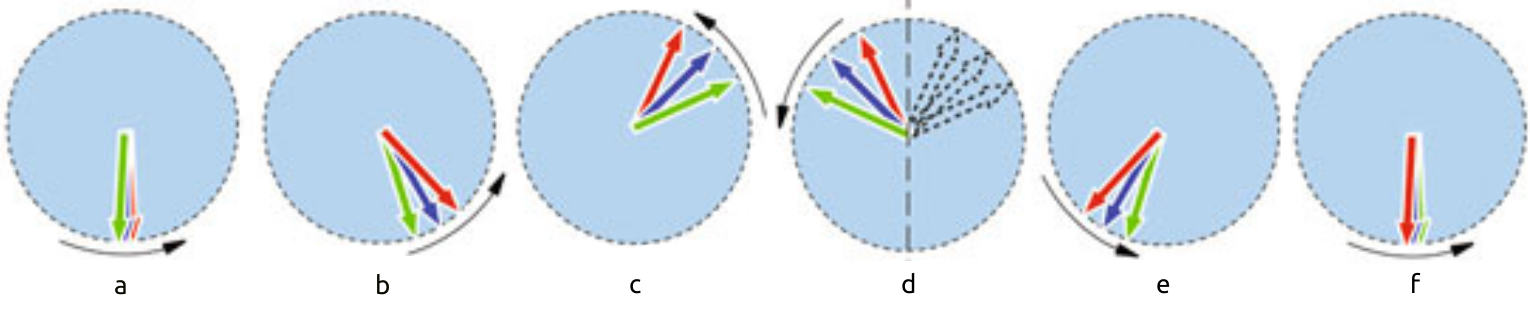
\includegraphics[width=1\textwidth]{images/t2_relax.png}
   \caption{(a) After the end of the 90° RF impulse the protons are with the same phase. (b) The protons precession are different due to the inhomogeneities of the magnetic field. (c) The phases are completely different, there are some faster protons than others. (d) A 180° RF impulse move the proton position in a symmetric way in order to the slower protons are after the faster. (e) In the rotation the spins recover progressively the same phase. (f) At this time is generated a spin echo. \cite{elementiRisonanza} Arranged.}
   \label{fig:T2_relax}
 \end{figure}

 \subsubsection*{Contrast}
 By varying $TE$ and $TR$, three types of contrast behavior can be obtained \ref{fig:matrixTR_TE}:
 \begin{itemize}
    \item $TE<<T_2$ and $TR=T_1$ : T\textsubscript{1}-contrast
    \item $TE=T_2$ and $TR>>T_1$ : T\textsubscript{2}-contrast
    \item $TE<<T_2$ and $TR>>T_1$ : $\rho$-contrast (proton density)
 \end{itemize}

 \begin{figure}[h]
    \centering
    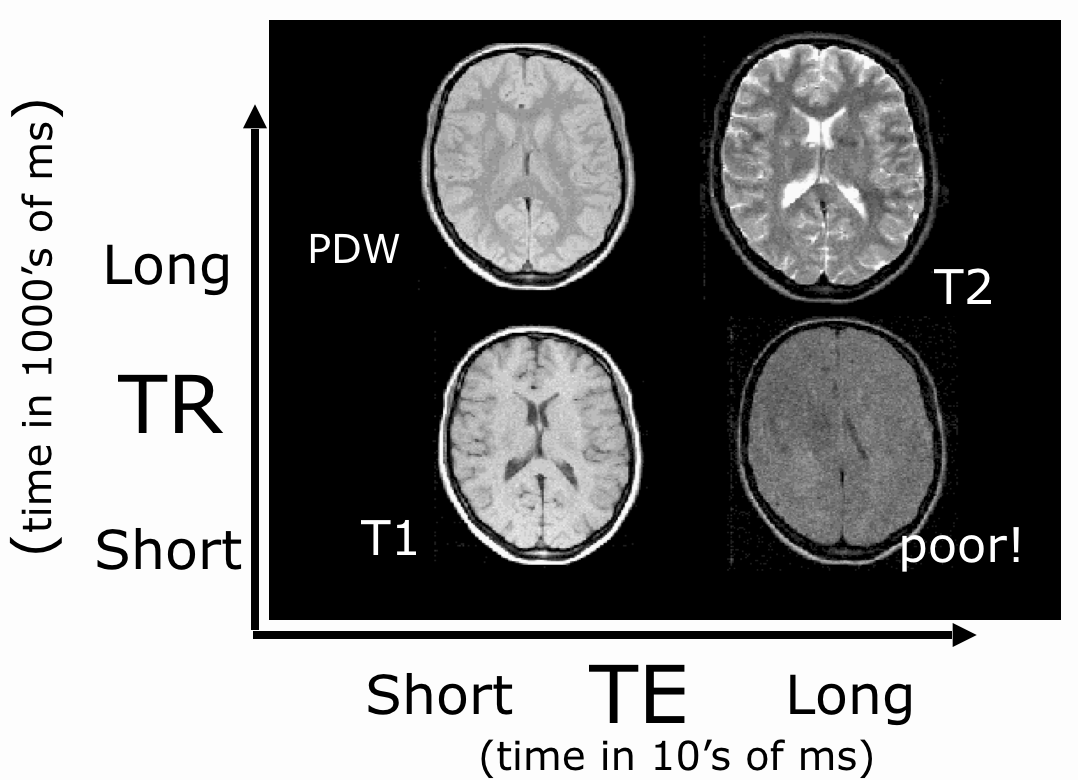
\includegraphics[width=0.8\textwidth]{images/matrix_contrast.png}
    \caption{Matrix showing the different contrasts obtained with different $TE$ and $TR$ values. \cite{matrixContrast}}
    \label{fig:matrixTR_TE}
 \end{figure}

 \subsection{Spatial coding}
 To reconstruct the image it is needed selecting a definite volume of tissue called \emph{voxel}\footnote{A voxel is the 3D expansion of a pixel}, three operations are needed to localize them in the tissue: selecting the layer (in the z-direction), selecting the column of the voxel (in the x-direction) and selecting the row (in the y-direction).
 These selections are done by linear variations of the magnetic field along a specific direction called \emph{Gradient fields}. They can change the static magnetic field $B_0$ and thus change the precession frequency of protons.\\
 
 \noindent To select a slice, it is applied a gradient along the z-direction, here the magnetic field change raising from a minimum to a maximum, and in the point in which the gradient is null the magnetic field is exactly $B_0$. Therefore only the nuclei in the condition of resonance will generate a signal \ref{fig:gradientZ}.

 \begin{figure}[h]
   \centering
   \begin{minipage}[c]{0.3\textwidth}
      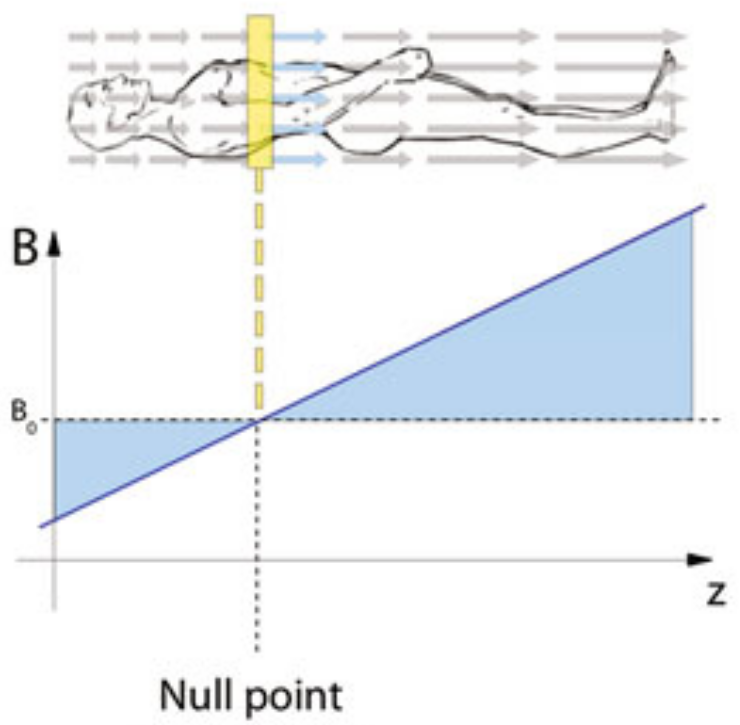
\includegraphics[width=\textwidth]{images/gradZ.png}
   \end{minipage}\hfill
   \begin{minipage}[b]{0.65\textwidth}
      \caption{The effect of the gradient $G_z$ is to resonate only the protons belonging to the slide in which the gradient is null (null point), only them have a field $B = B_0$ with a frequency equal to the Larmor frequency. \cite{elementiRisonanza}}
      \label{fig:gradientZ}
   \end{minipage}
 \end{figure}

 \noindent Using a gradient on the x-direction ($G_x$) creates a signal that is the \emph{sum of the associated signals with different frequencies}. This gradient is called \emph{Gradient of frequency encoding}, because the spins assume a precession frequency depending on the gradient. Successively, is applied a gradient along the y-direction ($G_y$), called \emph{Gradient of phase encoding}, it change the spin phase depending on the gradient \ref{fig:gradXY}. In this way each element of the section is different from the other by phase or frequency.

 The raw data from these signals are collected in matrices that represent the \emph{k-space} in the frequency domain, in which $G_y$ selects the row and $G_x$ scans it and save it in the matrix.
 This sequence must be repeated $n$ times for each line of the k-space to fill it \ref{fig:gradXY}.
 After, is applied the \emph{Inverse Fourier transform} to retrieve the image in the spacial domain.

 \begin{figure}[h]
    \centering
    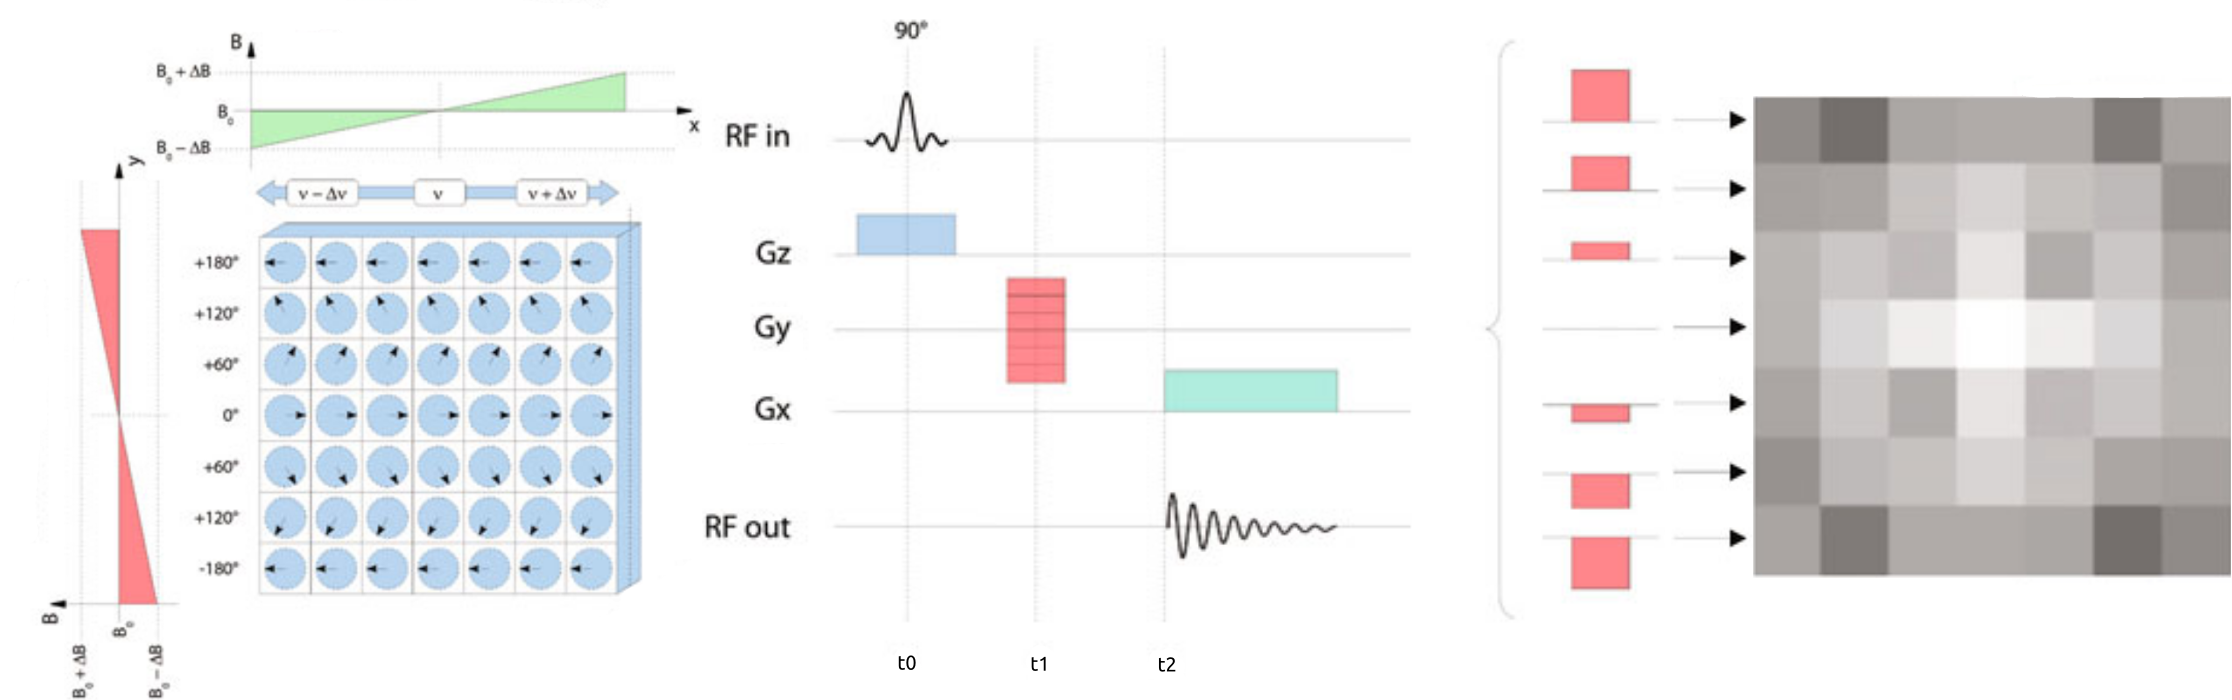
\includegraphics[width=1\textwidth]{images/gradxy.png}
    \caption{Gradients $G_x$ and $G_z$, temporal diagram and k-space. \cite{elementiRisonanza} Arranged.}
    \label{fig:gradXY}
 \end{figure}

 \subsection{Artifacts}
 In MRI artifacts is everything that is represented in the image without any correlation with the real anatomy of the tissues analyzed.
  \subsubsection*{Motion artifacts}
  The most common artifacts are the \emph{movement artifacts} due to the involuntary movements of the patient. In general the movements can be divided in random and periodic movements. Random movements create a blurring of the image, while periodic movements create \emph{ghost images}\footnote{Ghost images: periodic copies of some structures of the image}. The first can be reduced using techniques that reduce the acquisition time. The periodic movements artifacts can be reduced through \emph{gating}, a technique where the acquisition of the data is synchronized with the periodic movement of the tissue. \cite{artifacts}
  \subsubsection*{Magnet susceptibility artifacts}
  The presence of ferromagnetic materials create local inhomogeneities in the magnetic field which result in distortion artifacts called \emph{magnetic susceptibility artifacts}. The signals can change generating zone bright or dark with some distortions in the surrounding tissues. These artifacts can be reduced using spin-echo sequence instead of gradient-echo, and reducing the $TE$. \cite{artifacts}
  \subsubsection*{Chemical shift}
  In the interface between tissues of different molecular characteristics can occur a \emph{chemical shift}. It is a result of different resonance frequencies of adjacent tissues. Possible solutions are the reducing of the voxel dimension, increasing the bandwidth or using fat-suppressed imaging. \cite{artifacts}
  \subsubsection*{Gibb's artifacts}
  \emph{Gibb's artifacts} are due to the reconstruction from k-space, since it is performed through a finite sampling. In hedges of high-contrast the Fourier transform truncate some frequencies, for this they are also named \emph{truncation artifacts}, creating the effect of fine parallel lines ("ringing") adjacent to such interfaces. Increasing the matrix size or applying smoothing filters can reduce the artifacts. \cite{artifacts}
  \subsubsection*{Aliasing}
  \emph{Aliasing artifacts} are visible when the tissue is outside the field-of-view (FOV), meaning that there was an under-sampling in the k-space. The only solution is to increase the size of the FOV or using techniques of foldover suppression. \cite{artifacts}
  \subsubsection*{Eddy currents}
  The Faraday-Lenz Law of electromagnetism states that electrical currents (\emph{Eddy currents}) are induced in nearby conductors by a changing magnetic field. Since MRI uses rapidly changing magnetic fields, eddy currents are always produced. The conductive material in which eddy currents are induced may be any metallic component of the MRI scanner and the patient as a whole. These latter may generate a distortion of the magnetic field. Several techniques are available to minimize te effects including image post-processing \cite{QeA_MRI}.

  \begin{figure}[h]
     \centering
     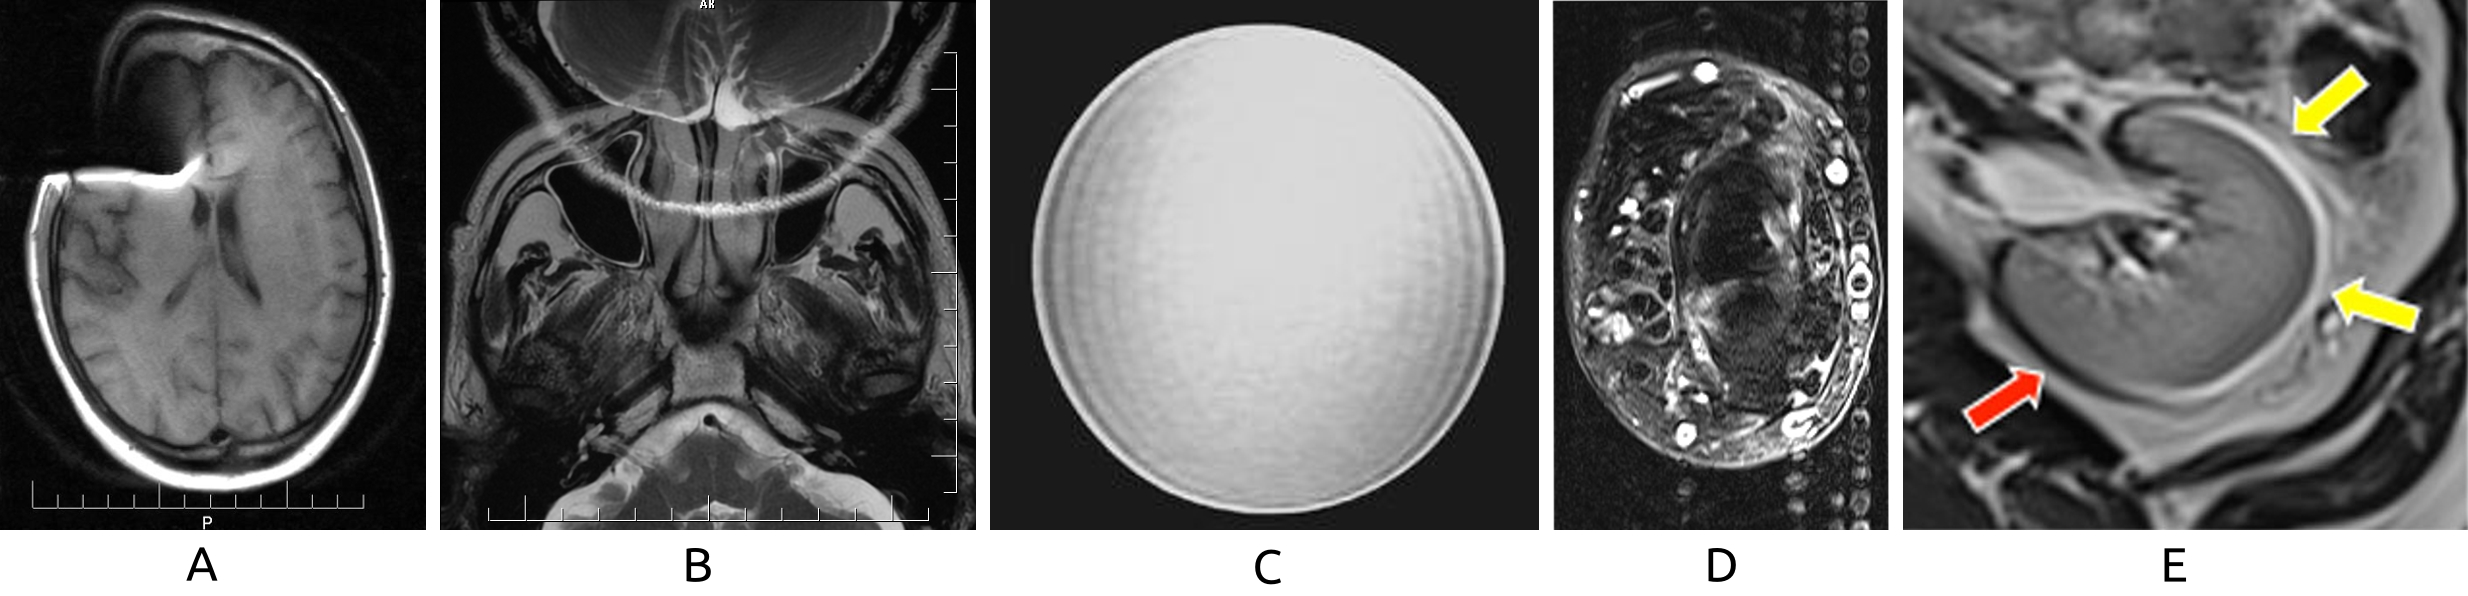
\includegraphics[width=1\textwidth]{images/artifacts.JPG}
     \caption{MRI artifacts: (A) Magnet susceptibility,; (B) Aliasing; (C) Gibb's ringing; (D) Chemical shift; (E) Chemical shift. \cite{artifacts} Arranged.}
     \label{fig:artifacts}
  \end{figure}

\section{Diffusion-Weighted MRI}
 Sequences of \emph{Diffusion-Weighted MRI} (DW-MRI) can provide motion-dependent contrast of water molecules in tissues, which can significantly alter in some brain diseases. This sequences are also know as \emph{Diffusion Weighted Imaging} (DWI) or \emph{diffusion MRI} (dMRI). 
 \subsection{Pulse Gradient Spin Echo (PGSE)}
 The \emph{Pulse Gradient Spin Echo} (PGSE) sequence is the main diffusion-weighted sequence used, it is composed of two magnetic gradients, before and after the 180° RF-pulse of the classic spin echo sequence. When the first diffusion gradient is applied, the water molecules are dephased, the second gradient, after the 180° RF pulse, will rephase the magnetization \ref{fig:PGSE}. The difference of gradient intensity which is subject the water molecule is proportional to the distance traveled on the time between the two gradients and also the gradient intensity. Therefore, the protons that are moved faster will have a greater dephase.\cite{elementiRisonanza}

 % sulle equation cita Resonnet 209
 The intensity of a voxel can be described by the Stejskal-Tanner equation as defined in \cite{dtiBook}, in which the signal will be equal to the intensity of a T\textsubscript{2}-weighted image, lowered by a quantity that depends on the diffusion of the molecules.
 \begin{equation}
    I = I_0 \cdot e^{-b_{PGSE} \cdot D}
 \end{equation}
 where $I$ is the intensity of received signal, $I_0$ is the intensity of base signal (T\textsubscript{2}-weighted), $b_{PGSE}$ is the factor of sensibility (parameters of PGSE sequence) and $D$ is the coefficient of diffusivity (intrinsic characteristic of the tissue).
 \begin{equation}
    b_{PGSE} = (\gamma G \delta)^{2}(\Delta - \frac{\delta}{3}) [s/mm^2]
 \end{equation}
 where $G$ is the diffusion gradient intensity, $\delta$ is the duration of the diffusion gradient and $\Delta$ is the time between the first diffusion and the second.

 \begin{figure}[h]
    \centering
    \begin{minipage}[c]{0.70\textwidth}
      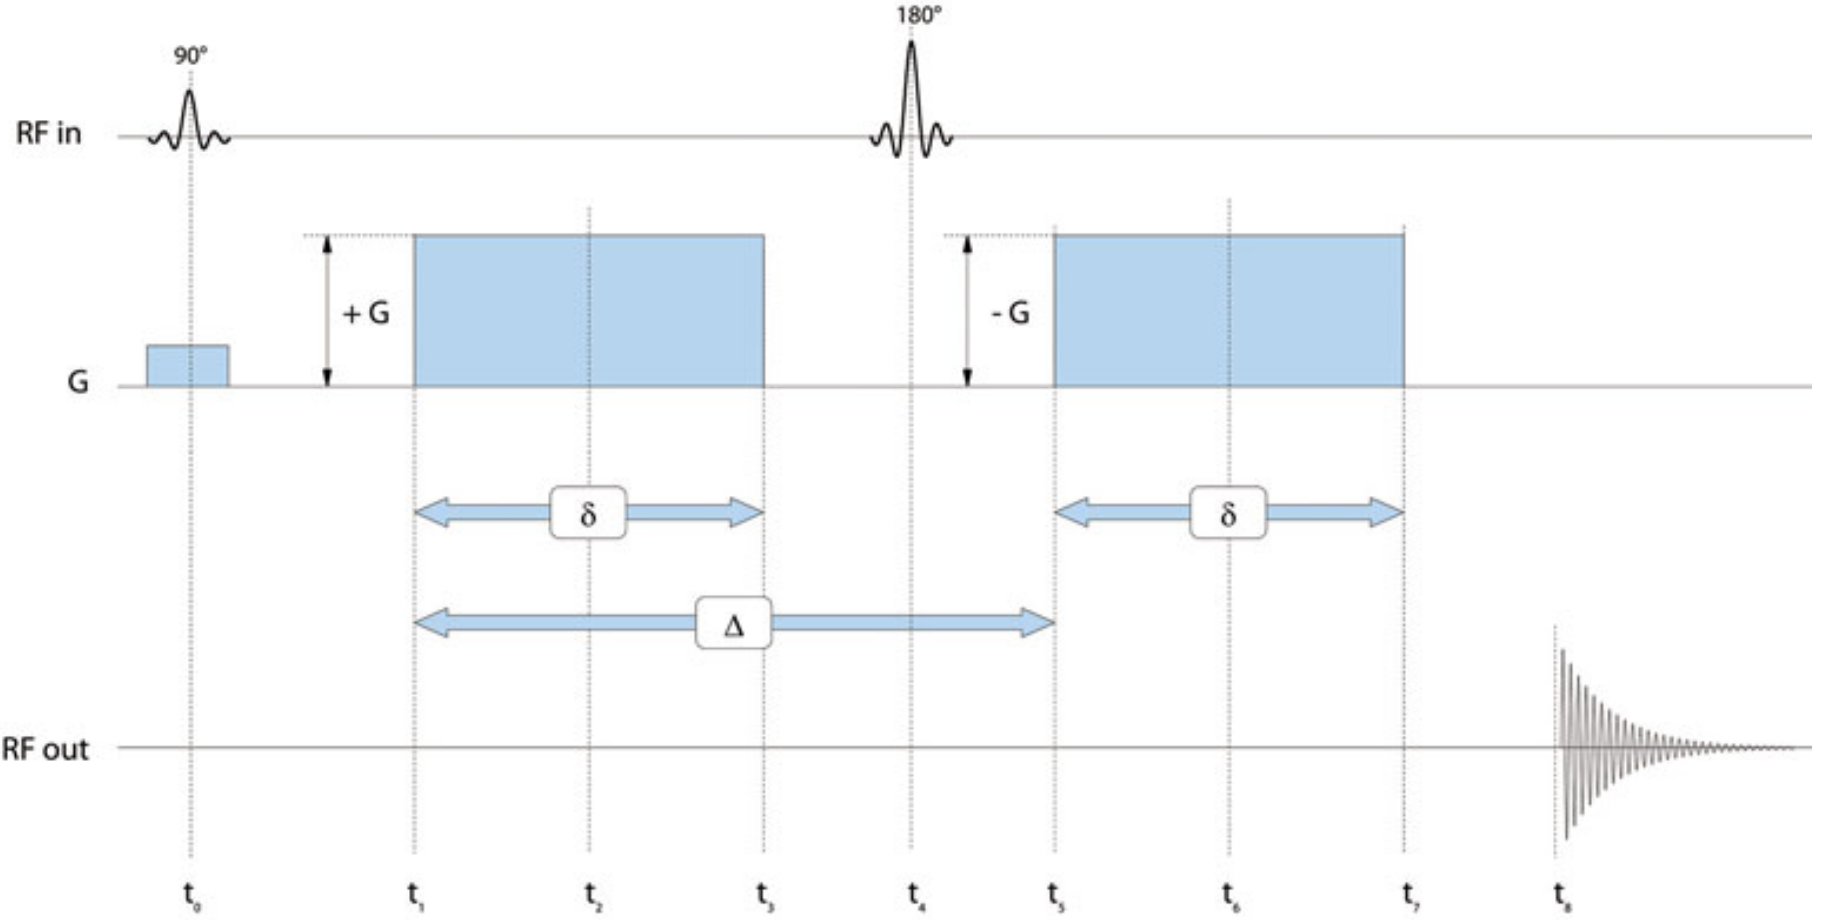
\includegraphics[width=\textwidth]{images/PGSE.png}
    \end{minipage}\hfill
    \begin{minipage}[c]{0.25\textwidth}
      \caption{Between the two diffusion gradients is present the 180° RF pulse, therefore the second gradient is equal to the first one, because the spin was already flipped by the 180° RF pulse. \cite{elementiRisonanza}}
    \label{fig:PGSE}
    \end{minipage}
 \end{figure}

 The diffusion can be affected even to pressure, temperature and molecular interactions and the DW-MRI can not distinguish between these different causes. Furthermore, if the followed path during the diffusion is random rather than linear, the signal will be only a measure between the starting point and the end point. For these reasons the $D$ is not correct and should be replaced by a coefficient called \emph{apparent diffusion coefficient} ($ADC$) \cite{elementiRisonanza}.
 \begin{equation}
    I = I_0 \cdot e^{-b_{PGSE} \cdot ADC}
 \end{equation}

 In the brain, the diffusivity of the water molecules is \emph{anisotropic}, it is not equal in each direction of the space. For example the diffusion in the white matter will be higher along the direction of the axons rather than the perpendicular direction. While, if the diffusion does not have any preferential direction, such as in the CSF, the diffusion is called \emph{isotropic} \ref{fig:isotropiAnisotropi}. In this case the Stejskal-Tanner equation as defined in \cite{dtiBook} becomes:
 \begin{equation}
    I = I_0 \cdot e^{-b_{PGSE} \cdot \hat{g}^T\mathbf{D}\hat{g}}
 \end{equation}
 where $\hat{g}$ is the gradient direction vector.

 \begin{figure}[h]
    \centering
    \begin{minipage}[c]{0.4\textwidth}
      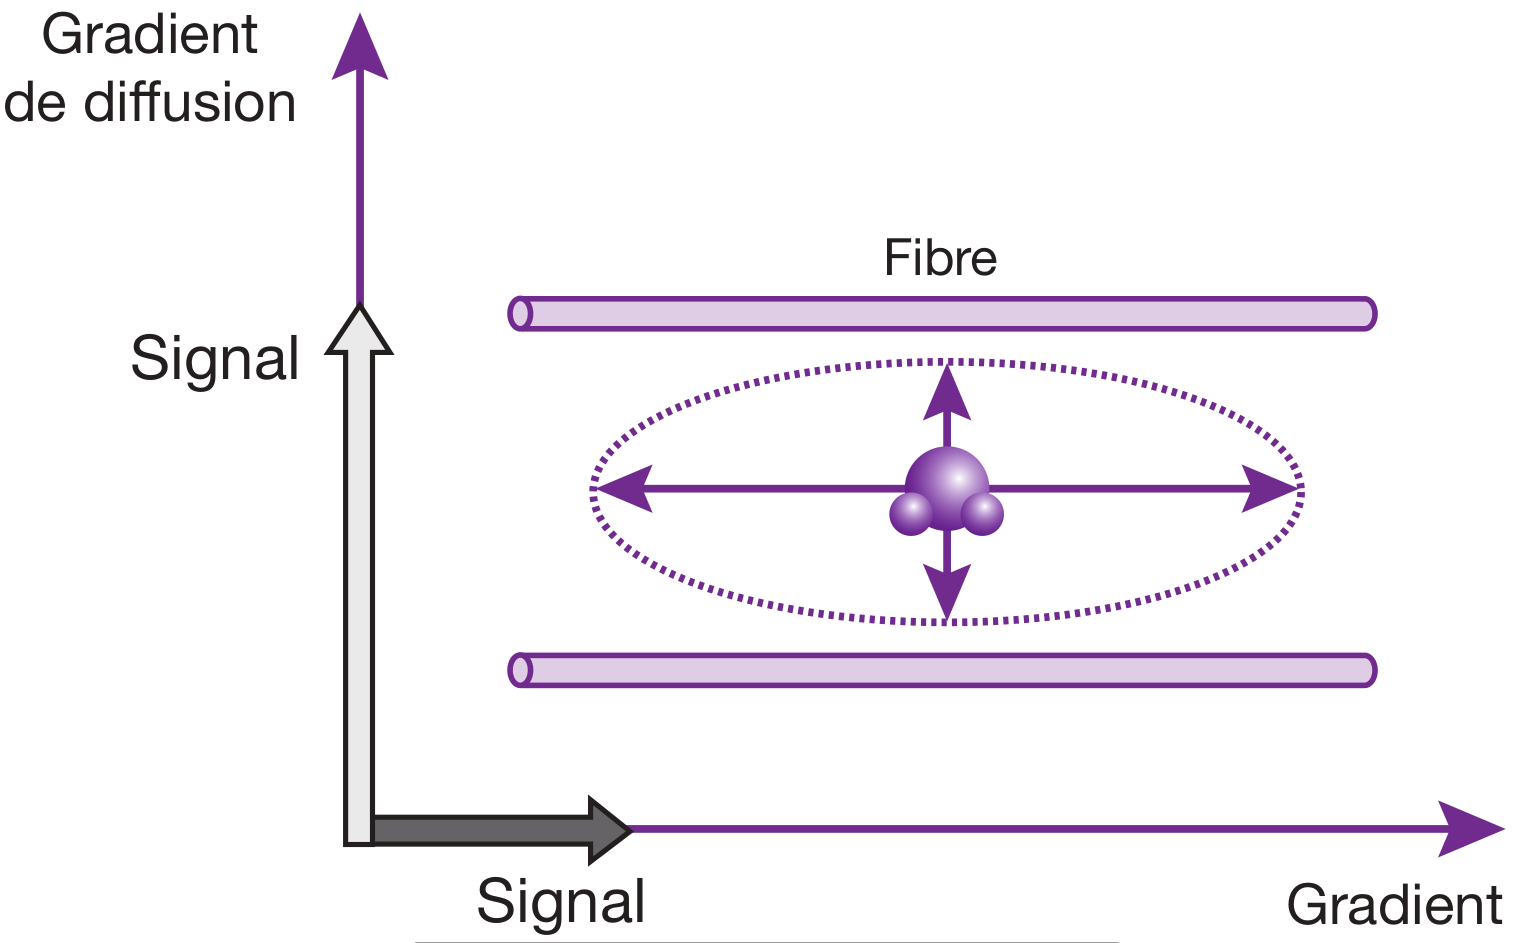
\includegraphics[width=\textwidth]{images/anisotropi.png}
    \end{minipage}\hfill
    \begin{minipage}[b]{0.5\textwidth}
      \caption{In the WM the diffusion of the water molecules is free along the axonal fibers, but it is reduced perpendicularly to the fibers. This is a case od Anisotropic diffusion. \cite{KastlerVetterIRM}}
      \label{fig:isotropiAnisotropi}
    \end{minipage}
 \end{figure}

 DWI collection involves setting a pre-determined number of gradient directions. That is, how many different angles within a 360-degree circle will water molecules be stimulated. For example, a DWI collection with 12 gradient directions will measure the diffusivity of water on every 30 degree angle, whereas a 32 gradient direction scan will measure every 11.25 degrees. \cite{de2011basic}

 \subsection{Diffusion Tensor Imaging (DTI)}
 One of the most popular and widely used mathematical models to describe the primary orientation of white math axonal path is called \emph{diffusion tensor imaging}. This model was introduced in 1994 \cite{basser1994mr} and it consists of estimating an effective \emph{diffusion tensor} ($\mathbf{D}$) within a voxel, which allows to represent its properties with a 3D ellipse. The diffusion tensor is described by a 3x3 symmetric tensor that uses 6 PGSE sequences, one for each different orientation of diffusion gradient, because $D_{yx}=D_{xy}$, $D_{zx}=D_{xz}$ and $D_{zy}=D_{yz}$.
 \begin{equation}
    \mathbf{D} = 
    \begin{pmatrix}
        D_{xx} & D_{xy} & D_{xz} \\
        \textcolor{gray}{D_{yx}} & D_{yy} & D_{yz} \\
        \textcolor{gray}{D_{zx}} & \textcolor{gray}{D_{zy}} & D_{zz}
    \end{pmatrix}
 \end{equation}

 Using the eigendecomposition of $\mathbf{D}$ are computed the eigenvectors and eigenvalues used to represent an ellipse on 3 orthogonal directions \ref{fig:elipse}. The eigenvalues $\lambda_{i}$ are the likelihoods of diffusion direction of a voxel. The largest eigenvalue($\lambda_1$) is the principal direction of axons in that voxel.
 \[\mathbf{D}=\mathbf{Q}\mathbf{\Lambda}\mathbf{Q}^{-1}\]
 \begin{equation}
    \mathbf{\Lambda} = 
    \begin{pmatrix}
        \lambda_{1} & 0 & 0 \\
        0 & \lambda_{2} & 0 \\
        0 & 0 & \lambda_{3}
    \end{pmatrix}
 \end{equation}

 \begin{figure}[h]
    \centering
    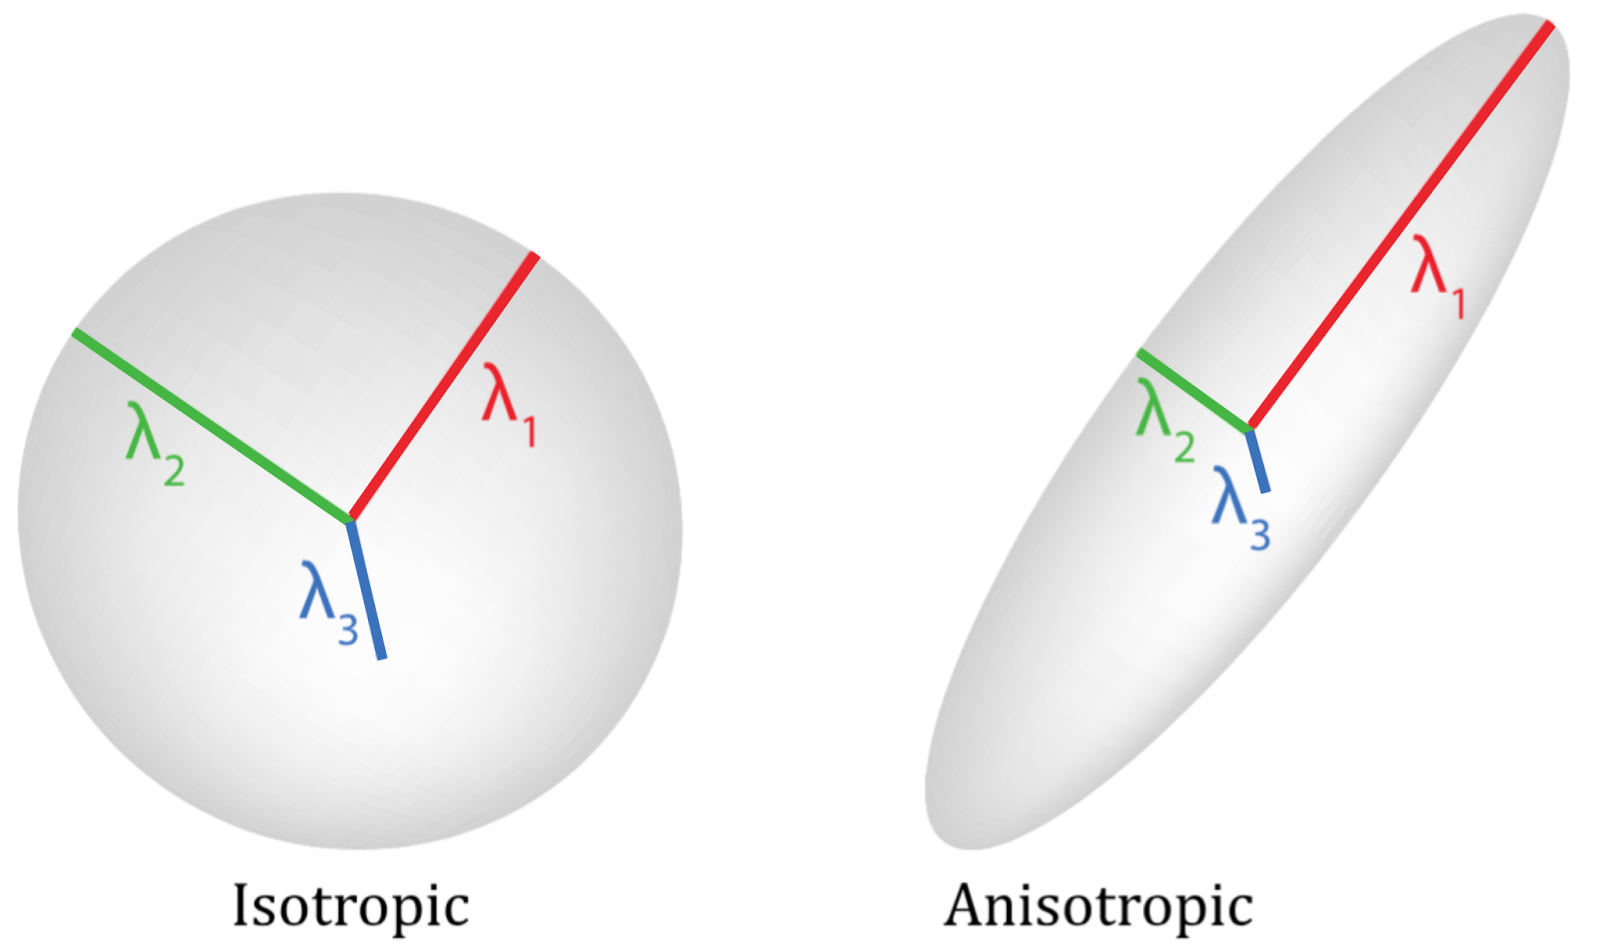
\includegraphics[width=0.4\textwidth]{images/ellipses.png}
    \caption{Isotropic and anisotropic tensor shapes, characterized by the eigenvalues of $\mathbf{D}$ ($\lambda_1$, $\lambda_2$, $\lambda_3$). \cite{ellipsoidDTI}}
    \label{fig:elipse}
 \end{figure}

 The result from the DW-MRI is difficult to visualize in a single image. In order to sintetize the information, the eigenvalues are used to compute some metrics that characterize each voxel. The most used are the \emph{Mean Diffusivity} ($MD$) and the \emph{Fractional Anisotropy} ($FA$) and they are computed by the $Trace$ of the diffusion matrix as defined in \cite{dtiBook}.
 \begin{equation}
    {MD} = \frac{{Tr}(D)}{3} = \frac{\lambda_1 + \lambda_2 + \lambda_3}{3}
 \end{equation}
 \begin{equation}
    FA = \sqrt{\frac{3}{2}}\frac{\sqrt{(\lambda_1-MD)^2+(\lambda_2-MD)^2+(\lambda_3-MD)^2}}{\sqrt{\lambda_1^2+\lambda_2^2+\lambda_3^2}}
 \end{equation}
 The $MD$ is proportional to the $Trace$ and it quantify the amplitude of the ellipse, or how much a particle is freely to move. Therefore, the $MD$ does not have any information about the directions, but on how much free water is contained into a voxel. The $FA$ is a metric between 0 and 1 and it measures the degree of anisotropy in a voxel. More the diffusion directions are equal more the $FA$ tends to 0. On the other and, an anisotropic diffusion will have a value of 1.
 
 % queste definizioni le ho prese direttamente dal book DTI.
 Other metrics are the \emph{Axial Diffusivity} ($AxD$) and the \emph{Radial Diffusivity} ($RD$), defined in \cite{dtiBook}. The Axial diffusivity is the diffusivity along the principal axis of the diffusion ellipsoid. While the Radial diffusivity is a measure used to express the diffusivity perpendicular to the principal direction of diffusion.
 \begin{equation}
    AxD = \lambda_1
 \end{equation}
 \begin{equation}
    RD = \frac{\lambda_2+\lambda_3}{2}
 \end{equation}

 Both $FA$ and $MD$ can be represented on \emph{diffusion direction maps}. The CSF will have an high $MD$ since the water is free to move in all the directions, while the WM will have an high $FA$ because oriented along a single direction. The image obtained from $FA$ is called \emph{FA map} and often they are displayed as \emph{RGB FA maps}, in which colors are used to represent the principal direction of the diffusion (Red: left-right; Green: anterior-posterior; Blue: superior-inferior) .

  \subsubsection*{Limitations of DTI}\label{section:dti_limitations}
  The main limitation of DTI model is that water molecules follow a Gaussian distribution. Therefore, only a bundle of fibers can be modeled inside each voxel, but in reality a complex organization of fibers is observed in every voxel. For example, a voxel containing two crossing fibers is modeled by a large diffusion tensor rather than two narrow tensors. Therefore in these voxel, the DTI model does not hold the assumption of a Gaussian distribution, and the resulting FA or MD metrics do not reflect the actual anatomical microstructure \ref{fig:fiber_crossing}. \cite{elementiRisonanza}

  \begin{figure}[h]
      \centering
      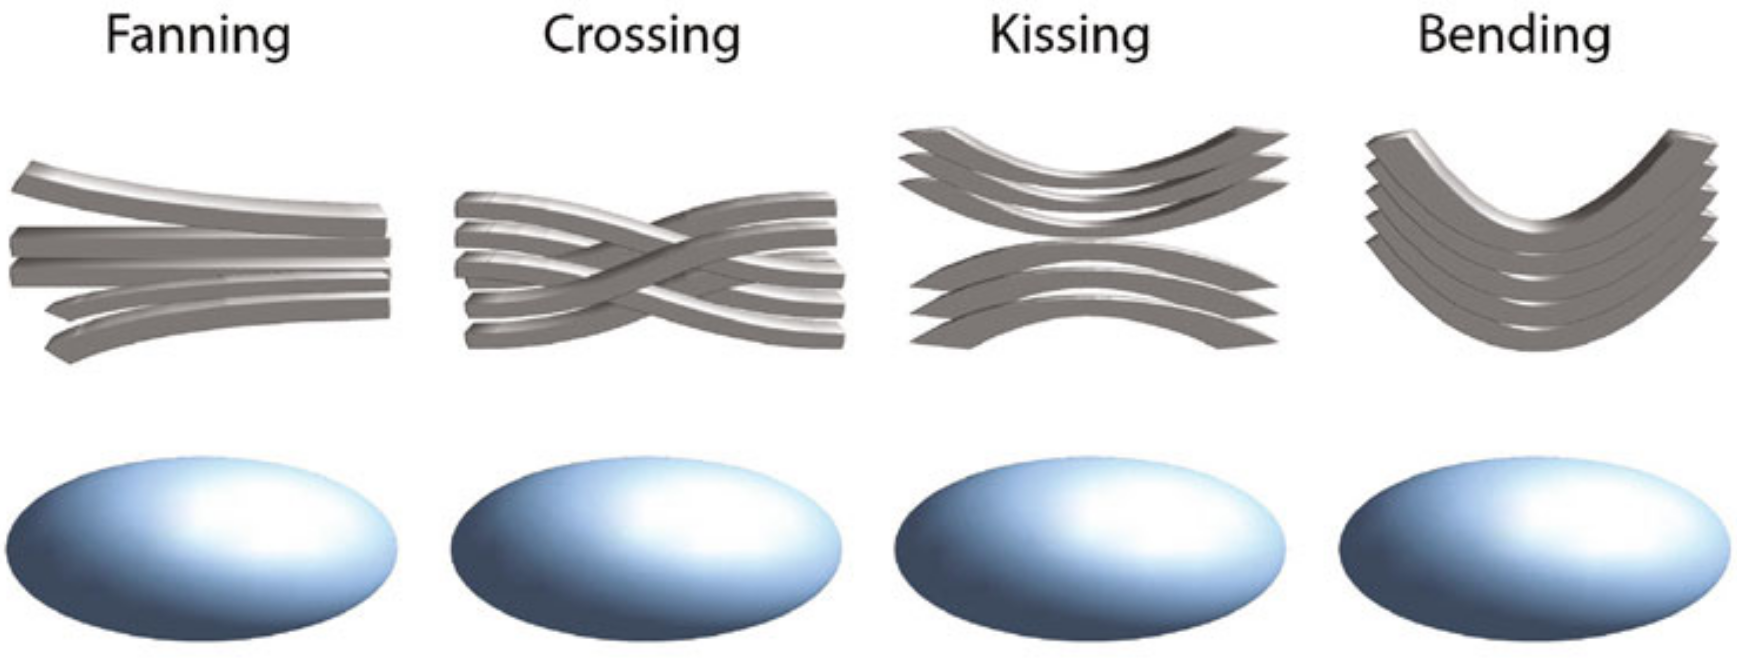
\includegraphics[width=0.8\textwidth]{images/fiber_orientations.png}
      \caption{In the cases of \emph{fanning}, \emph{crossing}, \emph{kissing}, \emph{bending} the DTI model is not capable to distinguish the differences. \cite{elementiRisonanza}}
      \label{fig:fiber_crossing}
  \end{figure}
 \subsection{Tractography}
 Tractography is a technique to estimate the pathways of the white matter fibers in the brain using data from DW-MRI. At the begin tractography was introduced by \cite{basser1998fiber} using his proposed DTI model \cite{basser1994mr} \cite{basser2011microstructural}. But, DTI assumes that white matter fibers have a single orientation (tensor) within each voxel, which can lead to false trajectory results in regions with crossing fibers, as explained in \ref{section:dti_limitations} and figure \ref{fig:fiber_crossing} \cite{basser2000vivo}. To resolve these limitation more advanced algorithms as CSD (\emph{Constrained Spherical Deconvolution}) \cite{tournier2007robust} are used.
 % Parlare dei algoritm, non parlare qua di MRtrxi 3 di quello se ne parlerà nei method usati

 CSD estimate the \emph{fiber orientation distribution} (FOD) from diffusion data. This distribution value provide information on other independent direction signal present within a voxel. In CSD model the signal $S(\theta, \phi)$ is assumed as convolution over the unit sphere \ref{fig:csv_conv} between the fiber orientation density function (FOD) $F(\theta, \phi)$ and the response function $R(\theta)$, as defined in \cite{tournier2004direct}: 
 \begin{equation}
   S(\theta, \phi) = F(\theta, \phi) \circledast R(\theta)
 \end{equation}

 \begin{figure}
   \centering
   \begin{subfigure}{.47\textwidth}
     \centering
     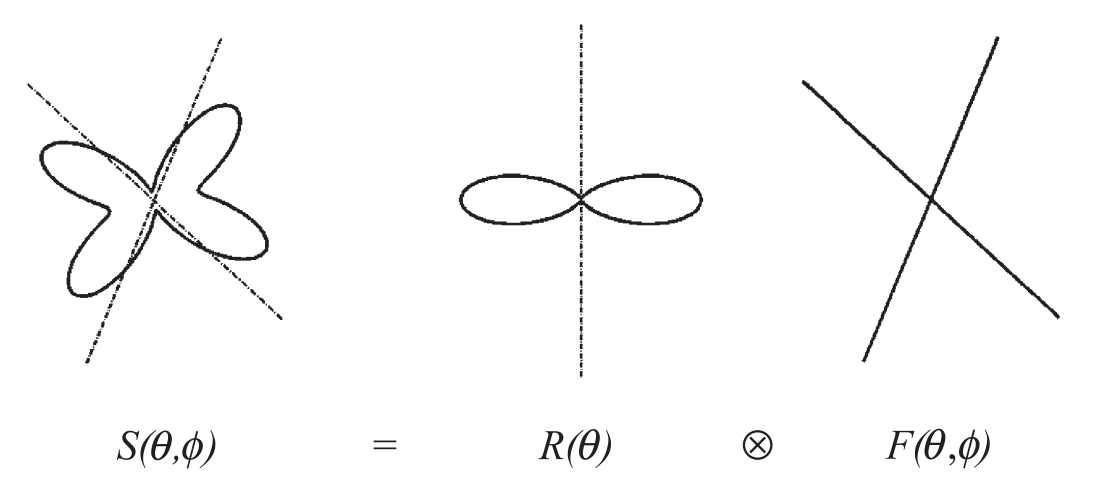
\includegraphics[width=\linewidth]{images/csv_conv.png}
     \caption{2D illustration of a voxel containing two fiber population. It can be expressed as a convolution over the unit sphere of an axially symmetric response function $R(\theta)$ with a fiber orientation density function $F(\theta, \phi)$. In this case $F(\theta, \phi) = \frac{1}{2}\delta(\theta_1, \phi_1)+\frac{1}{2} \delta(\theta_2, \phi_2)$. \cite{tournier2004direct}}
     \label{fig:csv_conv}
   \end{subfigure}\hfill
   \begin{subfigure}{.47\textwidth}
     \centering
     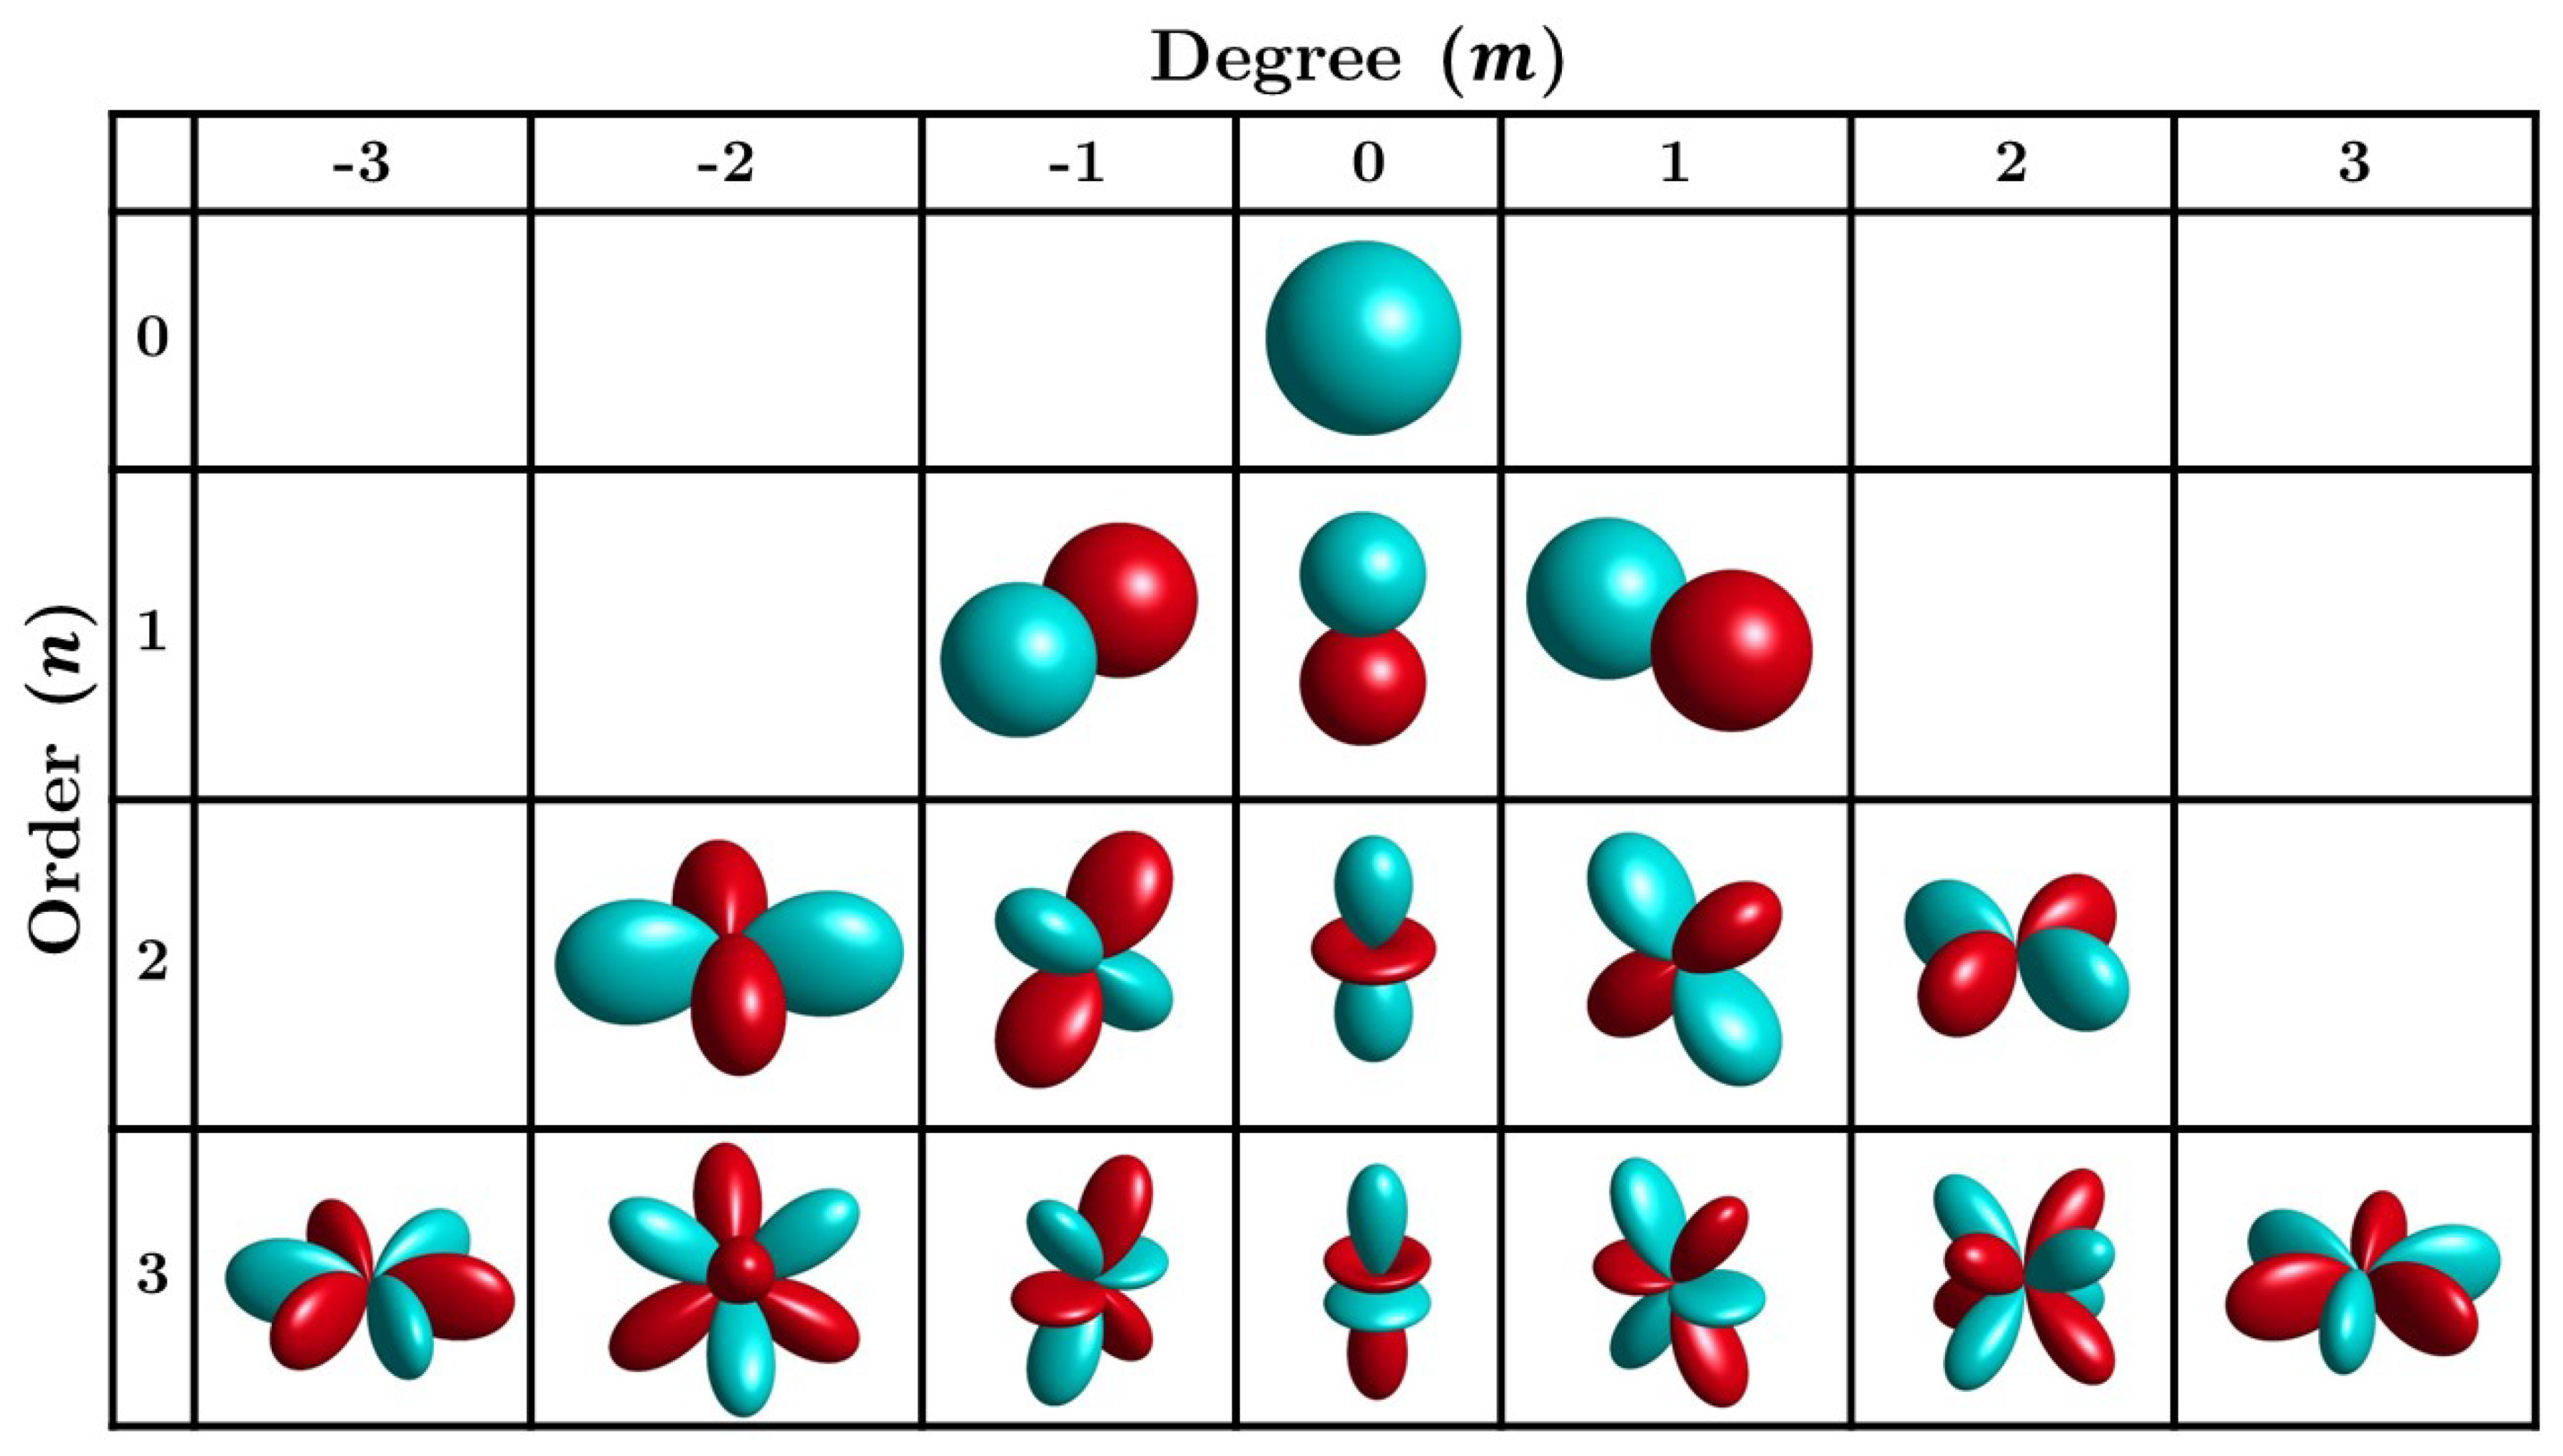
\includegraphics[width=\linewidth]{images/spherical_harmonics.png}
     \caption{ Real parts of the spherical harmonics up to third order ( $n=0,1,2,3$), for degree between $-3≤m≤3$, with lobes in cyan color indicating positive values and lobes in red color indicating negative values. \cite{e21060579}}
     \label{fig:spherical_harmonics}
   \end{subfigure}
\end{figure}

 % https://youtube.com/playlist?list=PLQN7oTTjz44SVSnMXDy66cFQrkm9a-jbw
  \noindent In order to estimate the FOD using CSD, it is first necessary to represent the FOD as a linear combination of \emph{spherical harmonic basis functions} \ref{fig:spherical_harmonics}. Then the fiber ODF $F(\theta, \phi)$ can be obtained by doing the \emph{spherical deconvolution} \cite{healy1998spherical}. 
 \\\\\\
 \noindent CSD supports only data acquired form a single shell\footnote{In diffusion MRI, a "shell" refers to a set of diffusion-weighted images acquired using the same b-value or a range of b-values. Multi-shell diffusion MRI refers to the acquisition of diffusion-weighted images using multiple b-values(e.g., b=0, b=1000, 2000, 3000 $s/mm^2$)}, and can provide high quality fODF estimates in voxel containing WM only, in other cases the results may be unreliable and noisy. In \cite{jeurissen2014multi} was developed a new model MSMT-CSD (\emph{Multi-shell Multi-tissue CSD}), which takes in account also extra-cellular and other tissues for each voxel.

 There are two different strategies used in fiber tractography: deterministic and probabilistic algorithms \ref{fig:det_prob_tract}. Both of them get as input diffusion data or a FOD, and starting from seed points they follow a preferred diffusion direction. \emph{Deterministic tractography} is a straightforward approach that involves tracking the dominant direction of diffusion at each voxel in the brain. However, deterministic tractography is sensitive to noise, crossing fibers (e.g. DTI model). \emph{Probabilistic tractography} models the distribution of possible pathways rather than a single deterministic solution, the resulting tractography is based on a probability distribution of possible pathways. Probabilistic tractography can provide a more robust estimate of the tracts in the brain (e.g. MSMT-CSD model). \cite{behrens2007probabilistic}

 \begin{figure}[h]
   \centering
   \begin{minipage}[c]{0.6\textwidth}
     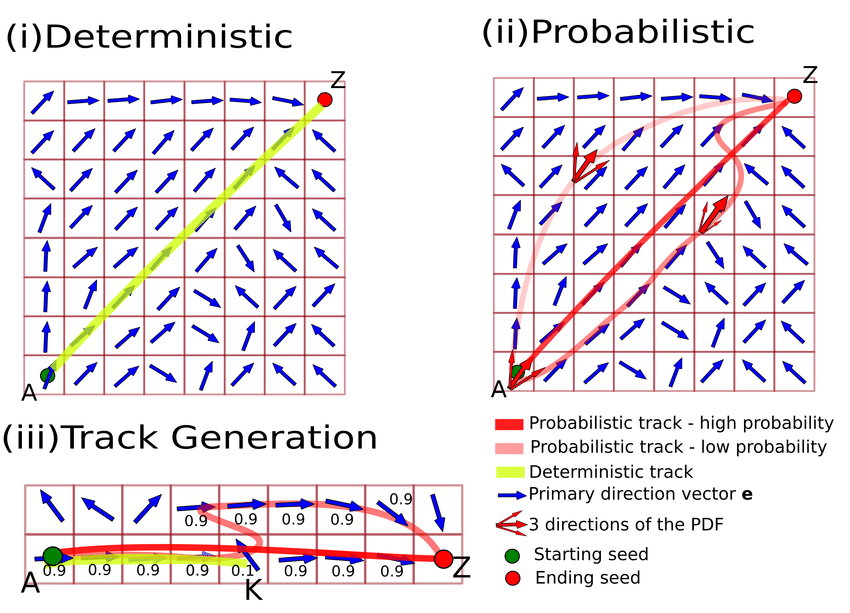
\includegraphics[width=\textwidth]{images/det_prob_tract.png}
   \end{minipage}\hfill
   \begin{minipage}[b]{0.37\textwidth}
      \caption{Basic example showing the difference between deterministic and probabilistic tracking models. \cite{phdthesisGaryfallidis}}
      \label{fig:det_prob_tract}
   \end{minipage}
\end{figure}

\section{DW-MRI Microstructural models}
 \subsection{NODDI}
 Dendrites and axons, known collectively as neurites, are the cellular building blocks of the computational circuitry of the brain. Quantifying neurite morphology in terms of its density and orientation distribution provides a view between normal populations and populations with brain disorder. \cite{zhang2012noddi}
 Neurite Orientation Dispersion and Density Imaging (NODDI) is a three-compartment tissue model that models the microstructure complexity of dendrites and axons. Such indices of neurites provide more specific markers of brain tissue microstructure than DTI. \cite{zhang2012noddi}
 \\\\
 NODDI distinguishes three types of microstructural environment: intra-cellular, extra-cellular and CSF compartments. Each gives to a separate normalized MR signal $A_i$ combined as
 \begin{equation}
   A=(1-\nu_{iso})(\nu_{ic}A_{ic}+(1-\nu_{ic})A_{ec})+\nu_{iso}A_{iso}
 \end{equation}
 where $A_{ic}$, $A_{ec}$, $A_{iso}$ and $\nu_{ic}$, $\nu_{iso}$ are the normalized signal and volume fraction of intra-cellular, extra-cellular and CSF compartments respectively.
 % Qua una foto de fa vedere i differenti tipi
 \begin{figure}[h]
   \centering
   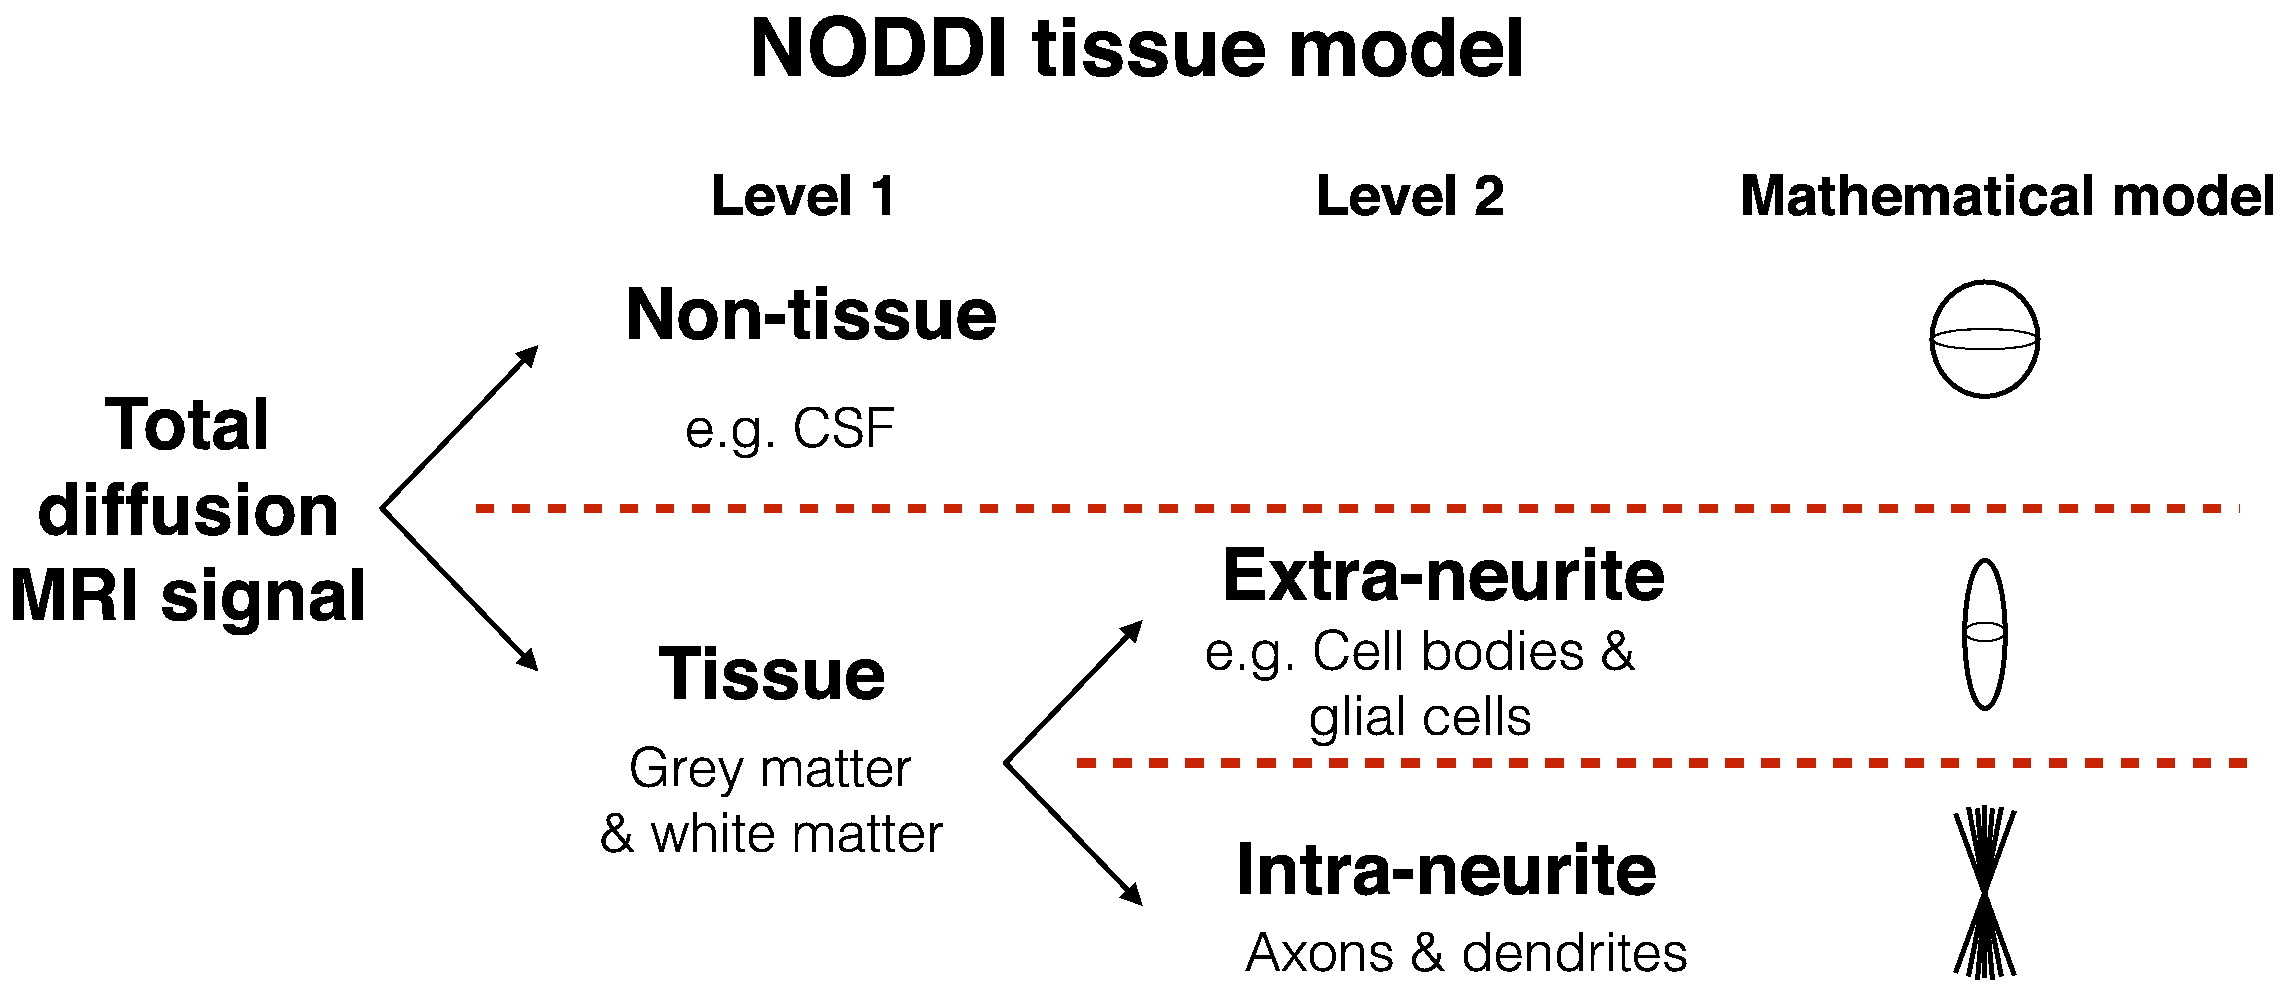
\includegraphics[width=0.70\textwidth]{images/noddi_tissues.jpg}
   \caption{Different compartments modelled by NODDI. The non-tissue compartment is modelled by isotropic Gaussian diffusion. The intra-neurite compartment models the neurites as orientationally dispersed sticks, while the space around the neurites is prescribed an anisotropic diffusion model. \cite{TARIQ2016207}}
   \label{fig:compartments}
 \end{figure}
 \\\\
 The \emph{intra-cellular} compartment refers to the space bounded by the membrane of neurites. This space is modeled by cylinders of zero radius (\emph{stiks}), and their orientation distribution can range from higly parallel to highly dispersed. The orientation distribution function is modeled with a \emph{Watson distribution}:

 \begin{equation}
   f(\mathbf{n}) = M(\frac{1}{2},\frac{3}{2},\kappa)^{-1}e^{\kappa(\mathbf{ \mu n})^2}
 \end{equation}
 where M is a confluent hypergeometric function, $\mu$ is the mean orientation, and $\kappa$ is the concentration parameter that measure the extent of orientation dispertion about $\mu$.
 The normalized signal, $A_{ic}$, is expressed as follows:
 \begin{equation}
   A_{ic} = \int_{\mathbb{S}^2} f(\mathbf{n})e^{-bd_{\parallel}(\mathbf{q\cdot n})^2} \,d\mathbf{n}
 \end{equation}
 where $\mathbf{q}$ and $b$ are the gradient direction and b-value of diffusion-weighting, $f(\mathbf{n})d\mathbf{n}$ gives the probability of finding stiks along orientation $\mathbf{n}$. $e^{-bd_{\parallel}(\mathbf{q\cdot n})^2}$ gives the signal attenuation due to unhindered diffusion along a stick with intrinsic diffusivity $d_{\parallel}$ and orientation $\mathbf{n}$.
 \\\\
 The \emph{extra-cellular} compartment refers to the space around the neurites which is occupied by varius types of glial cells and additionally gray matter and cell bodies \cite{zhang2012noddi}. The diffusion motion is modeled by a Gaussian anisotropic distribution and the normalized signal is modeled with a tensor since the perpendicular dissusivities are taken in account:
 \begin{equation}
   \log A_{ec} = -b\mathbf{q}^T(\int_{\mathbb{S}^2} f(\mathbf{n})D(\mathbf{n})\,d\mathbf{n})\mathbf{q}
 \end{equation}
 where $D(\mathbf{n})$ is the diffusion tensor with the principal diffusion direction $\mathbf{n}$, diffusion coefficients $d_{\parallel}$ and $d_{\perp}$ parallel and perpendicular to $\mathbf{n}$ respectively. The perallel diffusivity ($d_{\parallel}$) is the same as the intrinsic free diffusivity of the intra-cellular compartment, while the perpendicular diffusivity ($d_{\perp}$) is set as $d_{\perp} = d_{\parallel}(1-\nu_{ic})$.
 \\\\
 The CSF compartment models the space occupied by cerebrospinal fluid and is model as isotropv Gaussian diffusion with diffusivity $d_{iso}$.
 \begin{equation}
   A_{ios} = e^{-b d_{iso}}
 \end{equation}
  \subsection*{Model parameters}
  The complete set of parameters for the NODDI model is composed by: intra-cellular volume fraction ($\nu_{ic}$) also called \emph{Neurite Density Index} ($NDI$), parallel diffusion coefficient ($d_{\parallel}$), concentration parameter of Watson distribution ($\kappa$), mean orientation of Watson distribution ($\mathbf{\mu}$), isotropic volume fraction ($\nu_{iso}$), isotropic diffusivity ($d_{iso}$) \cite{zhang2012noddi}.
  The diffusivities are fixed to typical values\footnote{The diffusivities are fixed to respective typical values: $d_{\parallel}=1.7\times10^-3 mm^2s^{-1}$ and $d_{iso}=3\times10^{-3}mm^2s^{-1}$} and the remaining parameter are estimated. Furthermore, it is possible to compute the \emph{Orientation Dispersion Index} ($ODI$) \cite{zhang2011axon} which is a NODDI's summary statistic for quantifying angular variation of neurite orientation.
  \begin{equation}
   ODI = \frac{2}{\pi}\arctan(\frac{1}{\kappa})
  \end{equation}

  \subsubsection*{Limitations}
  NODDI focuses on explicitly modelling the fascicle dispersion with a Watson distribution of sticks in each voxel, but this assumption is inconsistent with the know tissue microstructure: fasciles with various microstructures have been observed in the brain. Furthermore it ignores the intra-axonal radial diffusivity and considers only a single fascicle compartment per voxel, while fascicles crossing with angle $>40\circ$ occurs in $60-90\%$ of the voxels. NODDI can capture crossing fascicles as increased dispersion but cannot characterize each of them separately. \cite{scherrer2016diamond}
 \subsection{DIAMOND}
 The signal arising from a voxel is composed by signals of multiple compartments. Model whose parameters reflect the tissue compartment present in each voxel are called \emph{diffusion compartment models} \ref{fig:multicompartment}. The \emph{DIstribution of 3D Anisotropic MicrOstructural eNvironments in Diffusion-compartment imaging} (DIAMOND) is an hybrid biophysical model of the tissues that combines multicompartment and statistal modelling to provide insight into each compartment in each voxel.\cite{scherrer2016diamond}. It is inspired by the statistical framework of \cite{yablonskiy2003} but capable to characterize the three-dimensional anisotropy of diffusion observed in the brain and describe the spin packets' distribution of fascicles. 

 % Qua che spiega i multi compartments
 \begin{figure}[h]
   \centering
   \begin{subfigure}{.32\textwidth}
      \centering
      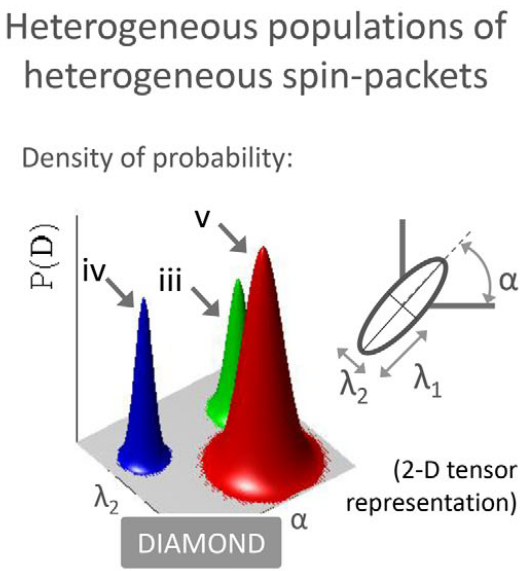
\includegraphics[width=\textwidth]{images/diamond1.png}
      \caption{}
      \label{fig:multicompartment}
   \end{subfigure}
   \begin{subfigure}{.32\textwidth}
      \centering
      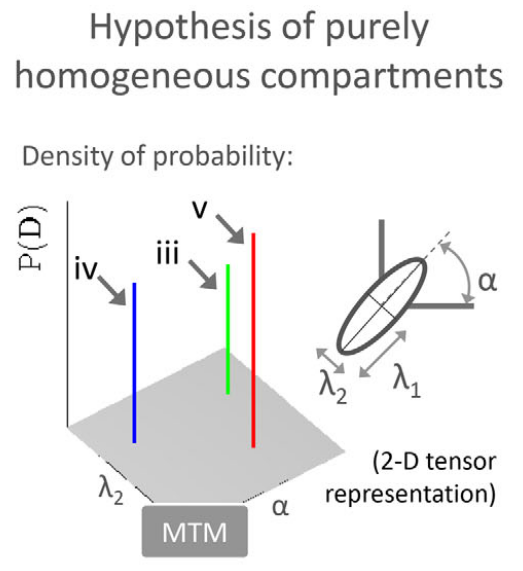
\includegraphics[width=\textwidth]{images/diamond2.png}
      \caption{}
      \label{fig:homogeneous_compartments_diamond}
   \end{subfigure}
   \begin{subfigure}{.32\textwidth}
      \centering
      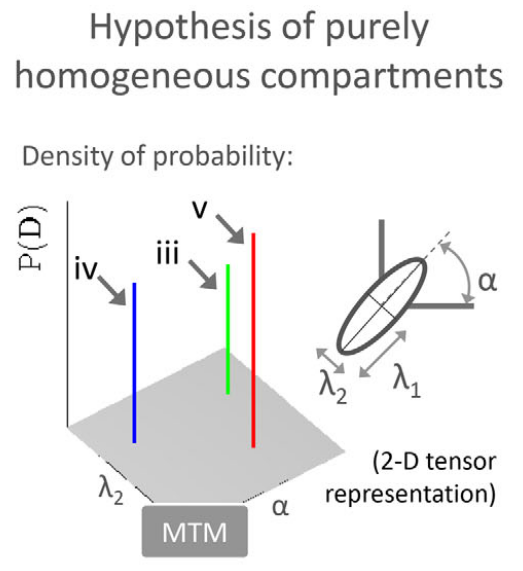
\includegraphics[width=\textwidth]{images/diamond3.png}
      \caption{}
      \label{fig:heterogeneous_compartments_diamond}
   \end{subfigure}
   \caption{(a) Example of a voxel in which an isotropic (red) and two anisotropic (blue and green) compartments are mixed; (b) The corresponding probability density function of diffusivities is composed of a mixture of delta functions; (c) Peak-shaped distributions of diffusivities. \cite{scherrer2016diamond}}
 \end{figure}

 DIAMOND requires the estimation of the number of tissue compartments in each voxel, which enables direct assesment of compartments-specific diffusion characteristic such as the compartment mean diffusivitu ($cMD$), axial diffusivity ($cAD$) and radial diffusivity ($cRD$). 
 \\\\
 The fraction of spin packets described by a 3D diffusivity $\mathbf{D}$ in the voxel is given by a \emph{matrix-variate} distribution $P(\mathbf{D})$. Therefore, if a voxel consisted of exaclty one \emph{homogeneous} microstructural environment characterized by a tensor $\mathbf{D}^0$, then $P(\mathbf{D})$ would be a delta function $P(\mathbf{D})=\delta(\mathbf{D}-\mathbf{D}^0)$ and the model would be equivalent to DTI. While, if it consisted of several identifiable homogeneus microstructural environments, a mixture of delta functions would be used \cite{scherrer2016diamond} \ref{fig:homogeneous_compartments_diamond}. Then the DW signal $S_k$ is modeled by:
 \begin{equation}\label{eq:1.26}
   S_k = S_0 \int_{\mathbf{D}\in Sym^{+}(3)} P(\mathbf{D})\exp(-b_k\mathbf{g}_k^T\mathbf{D}\mathbf{g}_k) \,d\mathbf{D}
 \end{equation}
 where $Sym^{+}(3)$ is the set of 3x3 SPD\footnote{SPD: symmetric positive-definite matrices 3x3} matrices, $\mathbf{g}_k$ is the orientation of the diffusion gradient and $b_k$ is the b-value of the sequence.

 More realistically each microstructural environment contain some degree of \emph{heterogeneity} and is best described by a \emph{population of spin packets}. To reach this by modelling each population with a peak-shaped matrix-variate distribution centred in $D^0$ \ref{fig:heterogeneous_compartments_diamond}. DIAMOND uses a \emph{matrix-variate Gamma} (mv-$\Gamma$) distribution with \emph{shape parameter} $\kappa > \frac{p-1}{2}$ and \emph{scale parameter} $\Sigma \in Sym^{+}(3)$ \cite{scherrer2016diamond}.
 \begin{equation}
   P_{\kappa,\Gamma}(\mathbf{D}) = \frac{|\mathbf{D}|^{\kappa-(p+1)/2}}{|\Sigma|^\kappa \Gamma_p(\kappa)}\exp (-trace(\Sigma^{-1}\mathbf{D}))
 \end{equation}
 where $|\cdot|$ is the matrix determinant and $\Gamma_p$ is the multi-variare gamma function. It's expectation is $\mathbf{D}^0=\kappa\Sigma$, and the shape parameter $\kappa$ determines the concentration of the densisty around the mean value $\mathbf{D}^0$. An heterogeneity index ($cHEI$) can be computed following the same transform as ODI in NODDI \cite{zhang2012noddi}: $cHEI(\kappa) = 2/\pi \arctan (1/\kappa)$.

 Considering $N_p$ populations each of them with a mv-$\Gamma$ distribution $P_{\kappa_j,\Sigma_j}(\mathbf{D})$ with $j \in [1,...,N_p]$ the matrix-variate distribution is defined as \cite{scherrer2016diamond}:
 \begin{equation}\label{eq:1.28}
   P(\mathbf{D}) = \sum_{j=1}^{N_p} f_j P_{\kappa_j,\Sigma_j}(\mathbf{D})
 \end{equation} 
 where $f_j$ are the occupation fractions and $\sum_{j=1}^{N_p} f_j = 1$. 

 Combining \ref{eq:1.26} and \ref{eq:1.28} and using the Laplace transformation, the following model is found \cite{scherrer2016diamond}:
 \begin{equation}
   S_k=S_0 \sum_{j=1}^{N_p} f_j \mathcal{D}(\mathbf{D}^0_j, \kappa_j)
 \end{equation}
 where $\mathcal{D}(\mathbf{D}^0,\kappa) = S_0 (1+\frac{b_k\mathbf{g}_k^T\mathbf{D}^0\mathbf{g}_k}{\kappa})^{-\kappa}$.

  \subsubsection*{Limitations}
  To summarise, DIAMOND focuses on capturing the distribution of 3D diffusivities arising from each tissue compartment (\emph{model of the tissues}), and in constrast of the \emph{model of the signal}, it requires the estimation of the number of tissue compartments ($N_p$) in each voxel, that is, the number of mv-$\Gamma$ components. The estimation of $N_p$ could be the only limitation of this model.
 \subsection{Microstructure fingerprinting}
 Microstructure fingerprinting is a model which leverages Monte Carlo simulation for the estimation of physically interpretable microstructural parameters, both in single and in crossing fascicles of axons in each voxel \cite{rensonnet2019towards}. It is a multicompartment model as DIAMOND, each voxel is composed of different structures. Monte Carlo simulations of DW-MRI signals, or \emph{fingerprints}, are pre-computed for a large collection of microstructural configurations. At every voxel, the microstructural parameters are estimated by optimizing a spase combination of the fingerprints \cite{rensonnet2019towards}.

 MF is based of the \emph{superposition principle} of crossing fascicles \ref{fig:superposition}, it assumes that the DW-MRI signal $S$ of each voxel is composed by independent contributions of $K$ fasciles of axons with different orientations $\mathbf{u}_k$ occupying fractions $\nu_k$ of the physical volume and of a partial volume $\nu_{CSF}$ of cerebrospinal fluid \cite{rensonnet2019towards}. $S$ can be espressed as:
 \begin{equation}
  \begin{aligned}
   S ={} & M_0 \left[ \sum_{k=1}^{K} \nu_k A_{fasc} ( \,\mathbf{\Omega}_k,\mathbf{T}_k,\mathbf{u}_k;\mathbf{g}) \, + \nu_{csf} A_{csf}( \,D_{csf}, \mathbf{T}_{csf};\mathbf{g}) \, \right] \\
    = & \sum_{k=1}^{K} w_k A_k + w_{csf}A_{csf} 
  \end{aligned}
 \end{equation}
 where $M_0$ is the initial transverse magnetization of the voxel, $A_k := A_{fasc} ( \,\mathbf{\Omega}_k,\mathbf{T}_k,\mathbf{u}_k;\mathbf{g}) \,$ is the normalized DW-MRI signal of the k-th fascicle, modeled by a Monte Carlo simulation, that would arise from an environment composed of fasciles with parameters $\mathbf{\Omega}_k$ and $\mathbf{T}_k$, and $w_k$ is its weight defined as \ref{eq:1.31}. Water is assumed to diffuse freely and isotropically with a scalar diffusivity $D_{csf}$.
 \begin{equation}\label{eq:1.31}
   w_k = M_0\nu_k \iff \nu_k = \frac{w_k}{\sum_{k=1}^{K+1} w_k}
 \end{equation}

  \begin{figure}[h]
   \centering
   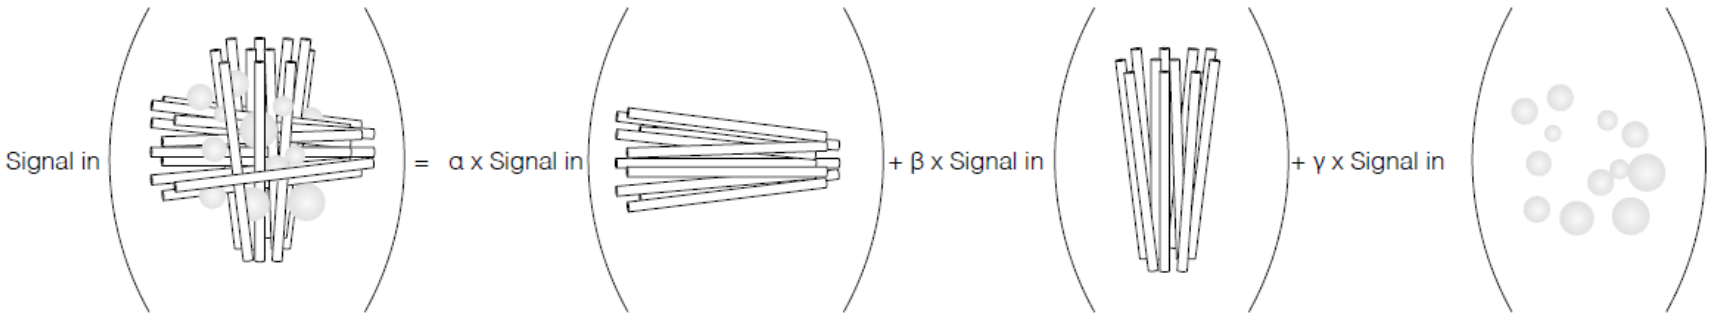
\includegraphics[width=0.8\textwidth]{images/superPosition.png}
   \caption{The toal signal is the sum of the attenuation of each compartments weighted by the respective volume fractions. \cite{rensonnet2015}}
   \label{fig:superposition}
 \end{figure}

 The dictionary is composed of DW-MRI signals (\emph{fingerprints}) obtained by Monte Carlo simulations of the random walk of water molecules in environments defined by \emph{hexagonal packing of impermeable cylinders} with different microstrucutral parameters $\Omega_k$ that rapresent the axons \cite{rensonnet2019towards}. The fasciles are modeled by an axonal radius ($r$) and separation between the cylinders ($s$) \ref{fig:hexagonal_packing}.

  % Qua 2.6 di Berger_brain anomalies  citarlo anche
  \begin{figure}[h]
   \centering
   \begin{minipage}[c]{.6\textwidth}
      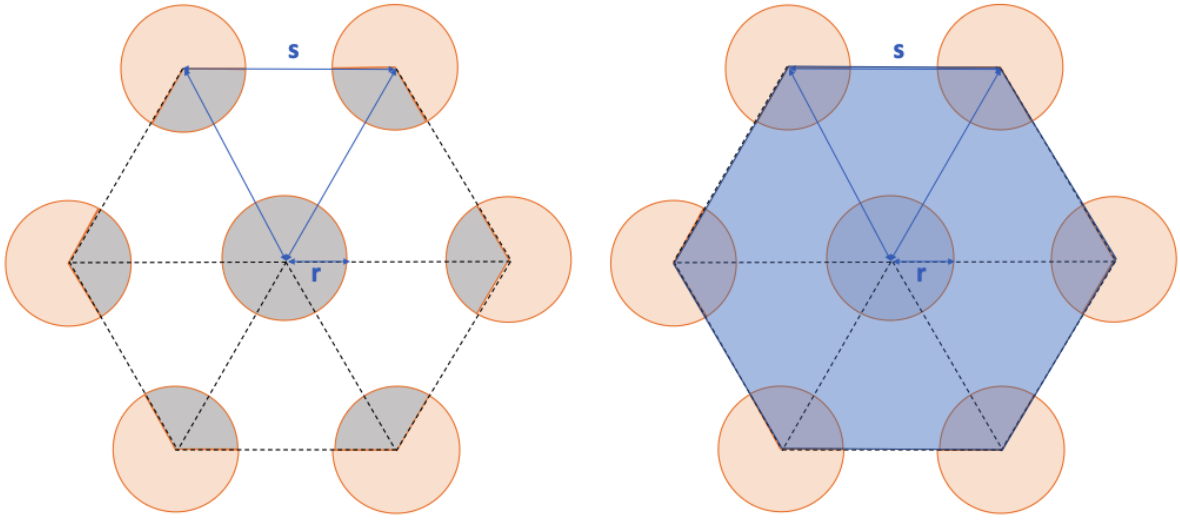
\includegraphics[width=\textwidth]{images/geometry_axons.png}
   \end{minipage}\hfill
   \begin{minipage}[c]{.35\textwidth}
      \caption{Rapresentation of hexagonal packing of cilinders. At left a rapresentation of the area of axons within the hexagon $A_{axons \subset hexagon}$, at the right the area of hexagon $A_{hexagon}$. \cite{berger2020} }
      \label{fig:hexagonal_packing}
   \end{minipage}
 \end{figure}

 \noindent Fascicle can be described by its intra-axonal volume fraction (or fiber volume fraction $fvf$), defined as ratio between the area of axons within the hexagon and the area of the hexagon \ref{eq:1.32}, and by extra-axonal diffusivity $D_{ex}$.
 \begin{equation}\label{eq:1.32}
   fvf_{fasc} = \frac{A_{axons \subset hexagon}}{A_{hexagon}} = \frac{2\pi}{\sqrt{3}} \left(\frac{r}{s}\right) ^ 2
 \end{equation}
 A canonical dictionary along the orientation $k=0$, $C^0 = \left[ A^0_1 \dots A^0_N \right] \in \mathbb{R}^{M \times N}$ is composed by concatenation of all the combinations of the possible fingerprints ($fvf$ and $D_{ex}$). \cite{dessain2022fast}
 \\\\
 After pre-computing the canonical dictionary, the optimal combination of configurations is found at runtime. The runtime method consist in concatenating all the rotations of $C_0$ along each population and then solving a \emph{sparse optimization problem} to find the best combination of fingerprint and orientation. The sparisty constraint ensure that only one fascicle is chosen out of all possible fascicle for a specific orientation \cite{rensonnet2019vivo}. The sparsity constraint problem can be defined as:
 \begin{equation}
   (\hat{j}_1, \dots, \hat{j}_K) = \argmin_{1\leq j_1, \dots, j_K \leq N} \min_{\mathbf{w}\geq0} \norm{ \mathbf{y} - \left[ \mathbf{A}^1_{j_1} | \dots | \mathbf{A}^K_{j_K} | \mathbf{A}_{csf} \right] \cdot \begin{bmatrix} w_1 \\ \vdots \\ w_K \\ w_{csf} \end{bmatrix} }
 \end{equation}
 where $\mathbf{y}$ is the measured signal, and $\mathbf{A}^k_{j_k} = \left\{ A_{fasc} \left( \Omega_{j_k},\mathbf{T}_k, \mathbf{u}_k;\mathbf{g}_i(t)\right) \right\}^M_{i=1}, 1\leq j_k \leq N $ is the signal from of a fascile with orientation $u_k$ and microstructural parameters defined with index $j$. Finally, $\hat{j}_k$ is the index of the optimal fingerprint in the k-th direction.\\
 From the optimal fingerprints and the weights is possible to extract the metrics by:
 \begin{align*}
 \nu_k = \frac{w_k}{\left(w_k + w_k\right)}; \; fvf_k = fvf_{\hat{j}_k}; \; D_{ex, k} = D_{ex, \hat{j}_k}
 \end{align*}

  \subsubsection*{Limitations}
  The use of the single scalars $r$ and $s$ to characterize the intra-axonal signal and the assumption on the impermeability of them is an overestimation of axons. Furthermore, the sparsity constraints do not allow mixtures of fingerprints to reconstruct the signal arising from a single fascicle of axons, this could be a limitation for fascicles with differrent microstructural properties in different sub-regions. \cite{rensonnet2019vivo}
